\chapter{Learning Constraints in Tabular Data}\label{ch:TaCLe}
Spreadsheets, comma separated value files and other tabular data representations are in wide use today.
However, writing, maintaining and identifying good formulas for tabular data and spreadsheets can be time consuming and error-prone.
We investigate the automatic learning of constraints (formulas and relations) in raw tabular data in an unsupervised way.
We represent common spreadsheet formulas and relations through predicates and expressions whose arguments must satisfy the inherent properties of the constraint. The challenge is to automatically infer the set of constraints that is present in the data, without labeled examples or user feedback. 
We propose a two-stage generate and test method where the first stage uses constraint solving techniques to efficiently reduce the number of candidates, based on the predicate signatures. 
Our approach takes inspiration from inductive logic programming, constraint learning and constraint satisfaction.
We show that we are able to accurately discover constraints in spreadsheets from various sources.

\section{Introduction}
% relevance of formulas and spreadsheets
Millions of people across the world use spreadsheets every day.
The tabular representation of the data is often intuitive, and the programming of functions in individual cells is quickly learned.
However, large and complex sheets, possibly with multiple tables and relations between them, can be hard to handle.
Many end-users lack the understanding of the underlying structures and relations in such sheets and the data they contain.
This is especially the case when spreadsheets have been exported from other software such as Enterprise Resource Planning (ERP) systems.
In this case, often a Comma Separated Values (CSV) format is used meaning that all formulas are lost, including inter-sheet formulas and relations.
%This limited understanding is especially the case with spreadsheets exported from other software such as ERP packages. In this case,
Even in manually created spreadsheets, it can be challenging to be consistent and correct with formulas across all tables.
For example, the influential Reinhart-Rogoff economical paper ``Growth in a Time of Debt'' \cite{growth_in_time_of_debt} had some of its claims contested~\cite{flaw_excel} after an investigation showed that the used Excel sheets contained mistakes in formulas.

% why learn them
\added{
Such issues and mistakes could be overcome through the development of intelligent user-assisting tools that would be able to automatically discover what constraints and formulas hold in a spreadsheet.
This is the problem we study in this chapter.
We envision that automatic constraint discovery can enable: auto-completion, error checking, formula suggestion, rich import and data compression.
Auto-completion can help users quickly populate spreadsheets by suggesting values for unfilled cells based on constraints that have previously been detected within the spreadsheet.
Error checking can identify erroneous values in spreadsheets, for example, while typing, by noticing that previously discovered constraint are violated by newly entered values, or offline by selectively leaving out values.
Both of these applications can facilitate the use of spreadsheets even for users who do not explicitly use formulas at all.
Furthermore, these applications are able to explain what constraints are responsible for suggesting or rejecting a value.
Other potential applications include formula suggestion, which is a variant of auto-completion that does not suggest a \emph{value} but provides a formula which computes the user provided value.
This setting can help users in finding the formula to perform a certain task or finding the right syntax for a formula.
Rich import denotes importing semi-structured data from another source such as CSV files and extracting the formula's that were used implicitly or explicitly.
A similar approach could be used to compress the data: instead of storing all data in a file, one can identify rows or columns generated by formula and store just that formula instead of the values.
%There are multiple applications that could build on this, such as rediscovery of constraints when importing raw data, auto-suggestion of formula's during spreadsheet use, automatic auto-completion of rows or columns, and consistency and error checking.
}

% why difficult
To this aim,  we investigate whether machine learning and knowledge discovery techniques can be used to learn constraints (formulas and other relations) in spreadsheet data in an unsupervised way.
From a machine learning point of view this is an unconventional problem because the data is in tabular form, but the constraints we wish to learn can involve both rows and columns of the table. Being unsupervised, there is no labeled information either, although for every possible function one can verify whether a certain input satisfies the definition.
%Unlike in other knowledge discovery tasks, such as pattern mining~\cite{}, there are many different types of formula and constraints we wish to discover, each with their own signature (number and properties of arguments) and definition.
From a data mining point of view, the data is relational on the one hand, since one can have multiple tables with relationships between them, but also consists of mixed textual and numeric types. More closely related is clausal discovery~\cite{claudien,lallouet}, learning CSP constraints \cite{QUACQ,Conacq,modelseeker} and dependency discovery in databases \cite{savnik}. But an important difference remains that we want to learn constraints on both columns and rows over integer, floating point as well as textual data.
Our inspiration comes from work on program synthesis, in particular Flashfill \cite{flashfill}, where the definition of a string-manipulation function is learned in spreadsheet data from very few examples.


% Moved up
The question that we ask in this chapter is: is it possible to learn the set of constraints present in a spreadsheet, from just tabular spreadsheet data? The main challenge is the number of possible constraints and combinations of rows and columns that need to be considered as input to the constraints.
To answer this challenge we propose a general-purpose method and system, named \sname (from: Tabular Constraint Learner, pronounced ``tackle''), for discovering row-wise and column-wise constraints. \added{Constraints on contiguous rows and columns are most common in spreadsheets, with semantically related items stored in rows or columns and formula's usually ranging over contiguous ranges, as formulas parallel to a table are often \textit{dragged} over its entire span.}
%
% contribs
Our contributions are as follows:
\begin{itemize}
\item we define the tabular constraint learning problem, where the goal is to find constraints that range over entire rows or columns in an unsupervised way;
\item we propose an effective two-stage generate-and-test method where the first stage reasons only over properties of contiguous blocks of rows/columns, and the second stage continues to investigate individual rows and columns and their content;
\item furthermore, in the first stage we use a constraint solver to efficiently enumerate all combinations of maximally contiguous blocks compatible with the arguments of the candidate constraints %, using backtracking search and forward checking;
\item experiments on different publicly available spreadsheets show that the system is able to extract constraints with high precision and recall.
\end{itemize}

%It operates directly on (headerless) tables of a spreadsheet in an unsupervised setting, that is, it reasons on raw tabular data directly with no example constraint instantiations given. %, and discovers column- and row-wise constraints.
%We demonstrate the utility of our approach in an experimental evaluation.
%Moreover, we sketch additional application scenario's such as autocompletion and error detection.


This chapter is organized as follows.
Section \ref{sec:tacle_related_work} discusses related work. Section \ref{sec:formalization} introduces the relevant concepts and defines the problem formally while Section \ref{sec:approach} presents our approach. This is evaluated in Section \ref{sec:evaluation} after which \added{we show how to realize two of the motivating applications using our system} in Section \ref{sec:applications}, and we conclude in Section \ref{sec:tacle_conclusions}.

%Due to the complexity of numeric computations in spreadsheets, people often fail to grasp the properties of the data, which leads to the so called Spreadsheet risk\footnote{\url{https://en.wikipedia.org/wiki/Spreadsheet\#Spreadsheet_risk}} and even caused major flaw in the famous economics papers \cite{flaw_excel} and billion-losses in the financial industry \cite{spreadsheet_risk_loss}. Tabular constraint learning provides a potential cure by indicating learned constraint violations and suggest possible fixes.

% {\it
% \textbf{Motivation}:
% \begin{itemize}
%   \item USED -- File generated from model, model got lost, need to reconstruct
%   \item Constraint programming is hard - is Excel hard?
%   \item Avoid manual analysis, provide selection of constraints
%   \item SOMEWHAT USED --Error checking
%   \item Completion, gain speed and insights (Complicated constraints, also complicated to verify, too much output)
% \end{itemize}

% \textbf{Novelty:}
% \begin{itemize}
%   \item USED -- Unsupervised setting (contrary to flashfill, etc)
%   \item Numeric, different constraints (contrary to single textual function solution in flashfill, etc)
%   \item USED -- Data format (2D) -- data is no longer in rows like a classic ML or DM settings
%   \item USED -- Declarative, general / modular, stacking of constraint problems
% \end{itemize}
%}
\section{Related Work}\label{sec:tacle_related_work}
\sname combines ideas from several existing approaches and different fields of research.

First, it borrows techniques from logical and relational learning \cite{luc_book}, as it discovers
constraints in multiple relations or tables. Unlike typical logical and relational learning
approaches, it focuses on data in spreadsheets and constraints involving both columns and rows in the sheets.
Furthermore, it derives a set of simple ``atomic'' constraints rather than a set of rules that each consist of a conjunction of literals as in clausal discovery \cite{claudien,lallouet}. Nevertheless, several ideas from logical and relational learning
proved to be useful, such as the use of a canonical form, a refinement graph, and pruning for redundancy. Tabular constraint learning also connects with the logical generalization of given formulas in a spreadsheet \cite{Isakowitz}, where the existing formulas are abstracted by introducing parameters in the place of particular cell references. The key difference here is that we discover constraints/formulas in the data, we do not have or use any prior information on the formulas in a spreadsheet.


Second, there exist a number of algorithms in the constraint programming community that induce constraints from one or more examples and questions. Two well-known approaches include ModelSeeker \cite{modelseeker} and Quacq \cite{QUACQ}.
The former starts from a single example in the form of a vector of values and then exhaustively looks for the most specific constraints that hold given a large constraint library. To this aim, it cleverly enumerates different de-vectorized tables; for instance, if the initial vector was of dimension $1 \times 20$, it would consider rearrangements of size $2 \times 10$, $4 \times 5$, $5 \times 4$, $\dots$ and Modelseeker would then look for both column, row  and even diagonal constraints. Key differences with our work are that we use spreadsheets with \textit{multiple} tables and that ModelSeeker's constraints are restricted to integer values and constraints that are typical for the constraint programming community, e.g., aimed at combinatorial optimization and scheduling. Conacq \cite{Conacq} acquires a conjunction of constraints using techniques inspired by Mitchell's version space algorithm to process examples; its successor Quacq uses active learning to query the user. Each of the examples/queries is processed for each constraint, hence an important issue is how fast the algorithm converges to the entire solution set (e.g. for Sudoku).
The focus is again on integer variables and typical combinatorial optimisation constraints. In a similar spirit the field of equation discovery \cite{equation_discovery} focuses, guided by  heuristics based on the structure of physical equations and unit measures, on the discovery of physical formulas over numbers and times series.
However, they focus specifically on noisy physical data and formulas, e.g., a single variable can take values from a series of measurements to get a regression parameter estimate or they apply specific data transformation such as numerical calculation of time and partial derivatives. In other words, the method works with approximations and the equation structures are heavily biased towards parameter estimation, while our goal is to discover hard constraints that hold over a subset of the rows and columns.
%As the conjunction for typical constraint programming problems (such as Sudoku) can be quite large, a key problem is to cope with redundant constraints. As Modelseeker, these systems focus on the types of constraints in combinatorial optimization but unlike ModelSeeker and our approach, they do not assume the variables are organized in tabular form.


Third, our work borrows from the seminal work of Gulwani et al. \cite{flashfill} on program synthesis for string manipulation in tabular data, which is incorporated in Microsoft's Excel. In FlashFill, the end-user might work on a table containing the surnames (column A) and names (column B) of scientists. The first row might contain the values A1 = ``Curie'' and B1 = ``Marie'', and the user might then enter in cell C1 the value ``M.C.''. At that point FlashFill generates a program that produces the output ``M.C.'' for the inputs ``Curie'' and ``Marie'', and also applies it to the other scientists (rows) in the table. While it might need an extra example to deal with names such as ``Bell'', ``Alexander Graham'' and determine whether it should output ``A.B.'' or ``A.G.B.'', FlashFill learns correct programs from very few examples. Flashfill has been extended to, e.g., FlashExtract \cite{flashextract} to produce a set of tables starting from an unstructured document (e.g., a txt or HTML file) with a set of examples marked for extraction. However, unlike our approach, Flashfill requires the user to identify explicitly the desired inputs/outputs from the function as well as to provide explicitly some positive and sometimes also negative examples.  In contrast, our approach is unsupervised, although it would be interesting to study whether it could be improved through user interaction and through user examples. \added{Furthermore, FlashFill handles only single tables with textual data to obtain a string transformation program, while the examples we consider contain multiple tables with mixed numeric and textual data and multiple constraints in them.} An interesting open issue for all of these techniques, with the exception of logical and relational learning, is how to deal with possibly incomplete or noisy data.

Fourth, also related to this line of research is the work on deriving constraints in databases such as functional and multi-valued dependencies \cite{savnik, Mannila-Raiha} although that line of research has focused on more specialized techniques for specific types of constraints. Many of the discovery techniques rely on the database schema~\cite{flach_dependency_discovery}, which is not available in our case. Techniques that work directly on the data have been investigated for the discovery of functional dependencies between attributes~\cite{tane_dependency_discovery}. The constraints and formulas we wish to learn go beyond that, including arithmetic, conditional arithmetic and \textit{fuzzy} lookups, for example.

Finally, worth mentioning is BayesDB \cite{BayesDB} and Tabular \cite{tabular}, two recent probabilistic modeling languages that have been specifically designed for dealing with relational data in tabular form and that can, as FlashFill, also automatically fill out missing values in a table.  However, unlike the other mentioned approaches, it is based on an underlying probabilistic graphical model that performs probabilistic inference rather than identify the ``hard'' constraints that hold in spreadsheets.


\begin{figure}[thb]

  \begin{subfigure}{1\textwidth}
  \begin{center}
    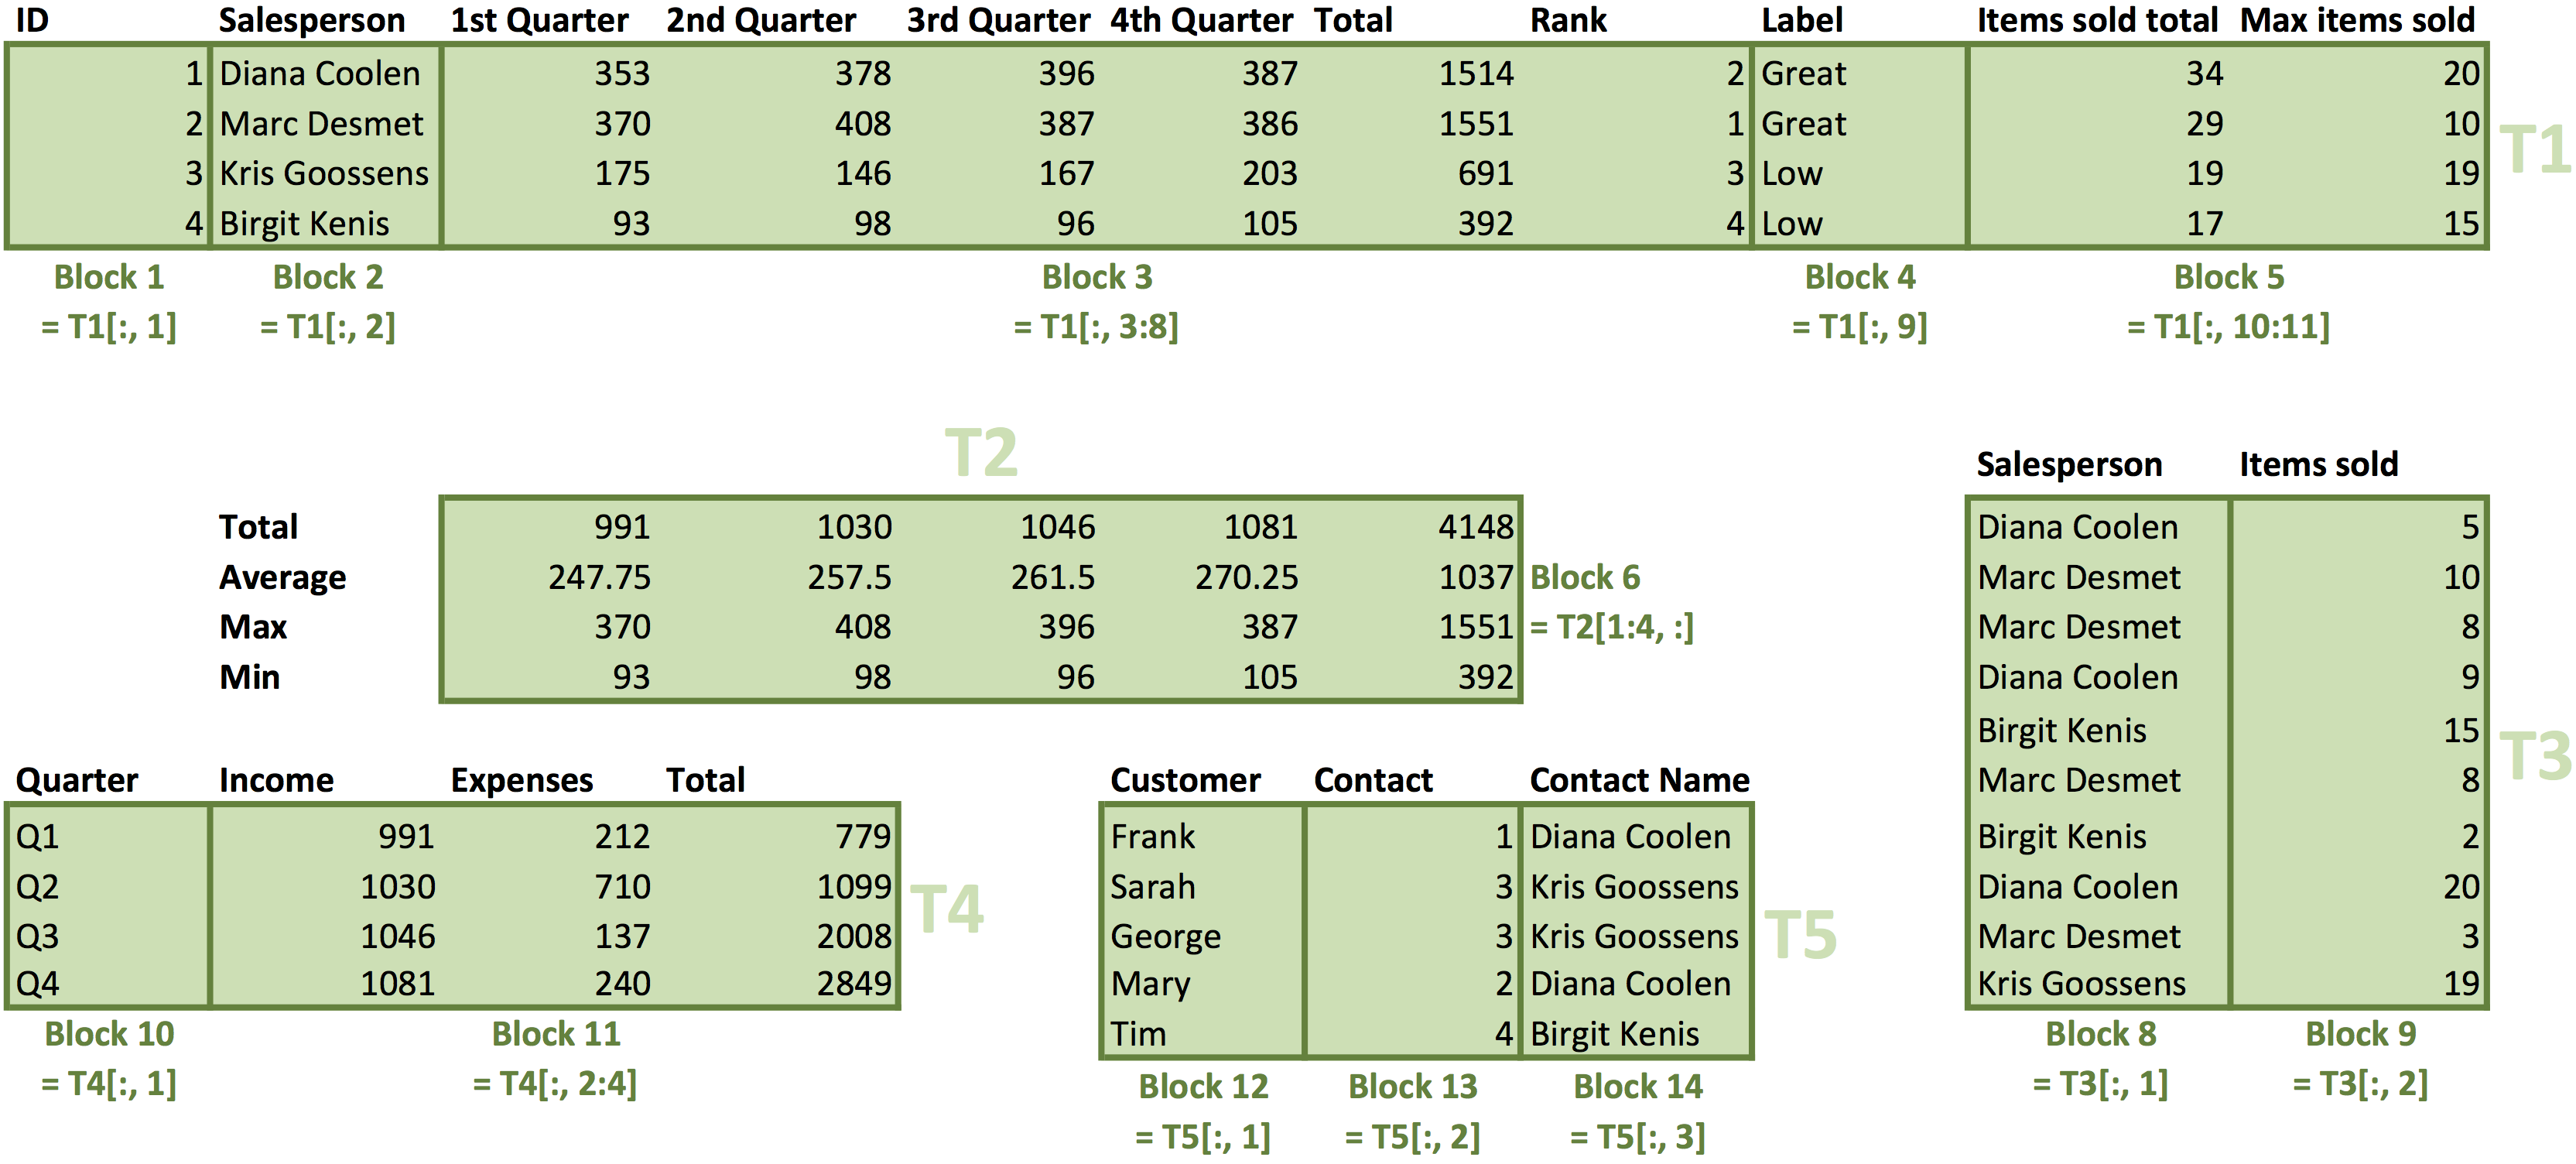
\includegraphics[width=1\textwidth]{Demo_full_block.png}
  \end{center}
  \vspace{-10pt}
  \caption{
    Example spreadsheet, black words and numbers only.
    Green background indicates headerless tables, dark borders indicate maximal type-consistent blocks.
    Most tables only contain type-consistent columns while table~$T_2$ also contains type-consistent rows. % (though its header indicates that it consists of row data).
%    However, due to the location of the header of~$T_2$ we can infer that it consists of row data.
    This example combines several Excel sheets based on exercises in the book ``MS Excel 2010''~\cite{excel_book}.
    % I guess you want to save space by having everything in one figure, but it might be useful to have a smaller figure on the first page just to explain this example in a bit more detail (or use a smaller example here); it's quite overwhelming now}
  }
  \label{fig:main_example}
\end{subfigure}
\hfill
\begin{subfigure}{1\textwidth}
  {\scriptsize
    \begin{align*}
      % Table 1
%
%      &~\ecperm{\range{T_{1}}{\rangeall}{1}}, \ecperm{\range{T_{1}}{\rangeall}{8}} \\
%
      &~\ecseries{\range{T_{1}}{\rangeall}{1}}                                  && \ecsumc{\range{T_{2}}{1}{\rangeall}}{\range{T_{1}}{\rangeall}{\rangeto{3}{7}}} \\
      &~\ecrank{\range{T_{1}}{\rangeall}{1}}{\range{T_{1}}{\rangeall}{5}}^*     && \ecaggc{\textit{AVERAGE}}{\range{T_{2}}{2}{\rangeall}}{\range{T_{1}}{\rangeall}{\rangeto{3}{7}}}  \\
      &~\ecrank{\range{T_{1}}{\rangeall}{1}}{\range{T_{1}}{\rangeall}{6}}^*     && \ecaggc{\textit{MAX}}{\range{T_{2}}{3}{\rangeall}}{\range{T_{1}}{\rangeall}{\rangeto{3}{7}}} \\
      &~\ecrank{\range{T_{1}}{\rangeall}{1}}{\range{T_{1}}{\rangeall}{10}}^*    && \ecaggc{\textit{MIN}}{\range{T_{2}}{4}{\rangeall}}{\range{T_{1}}{\rangeall}{\rangeto{3}{7}}} \\
      &~\ecrank{\range{T_{1}}{\rangeall}{8}}{\range{T_{1}}{\rangeall}{7}}       && \ecsumc{\range{T_{4}}{\rangeall}{2}}{\range{T_{1}}{\rangeall}{\rangeto{3}{6}}} \\
      &~\ecrank{\range{T_{1}}{\rangeall}{8}}{\range{T_{1}}{\rangeall}{3}}^*     && \range{T_{4}}{\rangeall}{4} = PREV(\range{T_{4}}{\rangeall}{4}) + \range{T_{4}}{\rangeall}{2} - \range{T_{4}}{\rangeall}{3} \\
      &~\ecrank{\range{T_{1}}{\rangeall}{8}}{\range{T_{1}}{\rangeall}{4}}^*    && \eclookup{\range{T_{5}}{\rangeall}{2}}{\range{T_{5}}{\rangeall}{3}}{\range{T_{1}}{\rangeall}{2}}{\range{T_{1}}{\rangeall}{1}}^*\\
%
      &~\ecsumr{\range{T_{1}}{\rangeall}{7}}{\range{T_{1}}{\rangeall}{\rangeto{3}{6}}}   && \eclookup{\range{T_{5}}{\rangeall}{3}}{\range{T_{5}}{\rangeall}{2}}{\range{T_{1}}{\rangeall}{1}}{\range{T_{1}}{\rangeall}{2}} \\
%
      &~\ecaggif{\textit{SUM}}{\range{T_{1}}{\rangeall}{10}}{\range{T_{3}}{\rangeall}{1}}{\range{T_{1}}{\rangeall}{2}}{\range{T_{3}}{\rangeall}{2}}   && \ecaggif{\textit{MAX}}{\range{T_{1}}{\rangeall}{11}}{\range{T_{3}}{\rangeall}{1}}{\range{T_{1}}{\rangeall}{2}}{\range{T_{3}}{\rangeall}{2}} 
%
    % Table 2
%     &~\ecsumc{\range{T_{2}}{1}{\rangeall}}{\range{T_{1}}{\rangeall}{\rangeto{3}{7}}} \\
%
%     &~\ecaggc{\textit{AVERAGE}}{\range{T_{2}}{2}{\rangeall}}{\range{T_{1}}{\rangeall}{\rangeto{3}{7}}} \\
%
%     &~\ecaggc{\textit{MAX}}{\range{T_{2}}{3}{\rangeall}}{\range{T_{1}}{\rangeall}{\rangeto{3}{7}}},  \\
%
%     &~\ecaggc{\textit{MIN}}{\range{T_{2}}{4}{\rangeall}}{\range{T_{1}}{\rangeall}{\rangeto{3}{7}}} \\
%
    % Table 4
%     &~\ecsumc{\range{T_{4}}{\rangeall}{2}}{\range{T_{1}}{\rangeall}{\rangeto{3}{6}}} \\
%
%     &~\range{T_{4}}{\rangeall}{4} = PREV(\range{T_{4}}{\rangeall}{4}) + \range{T_{4}}{\rangeall}{2} - \range{T_{4}}{\rangeall}{3} \\
%
    % Table 5
%     &~\eclookup{\range{T_{5}}{\rangeall}{2}}{\range{T_{5}}{\rangeall}{3}}{\range{T_{1}}{\rangeall}{2}}{\range{T_{1}}{\rangeall}{1}}^* \\
%
%     &~\eclookup{\range{T_{5}}{\rangeall}{3}}{\range{T_{5}}{\rangeall}{2}}{\range{T_{1}}{\rangeall}{1}}{\range{T_{1}}{\rangeall}{2}}
    \end{align*}}
  \vspace{-10pt}
  \caption{Constraints learned for the tables above, except 19 \textit{ALLDIFFERENT}, 2 \textit{PERMUTATION} and 5 \textit{FOREIGNKEY} and 5 \textit{\ecascname} constraints not shown.
  Constraints marked with $*$ were not present in the original spreadsheets.}
  \label{fig:sol_example}
\end{subfigure}
  \caption{Running example}
\end{figure}


\section{Formalization}\label{sec:formalization}
Our goal is to automatically learn the constraints that hold between the rows and/or columns in a spreadsheet. This is applicable not just to data from spreadsheets, but to any data in tabular form.

%An example spreadsheet with tables is given in Figure~\ref{fig:main_example}, we will use this as running example throughout the paper.

We first introduce some terminology and the concept of a \template, after which we define the problem and discuss some additional considerations.

\subsection{Terminology}
Spreadsheets and tabular data may conceptually consist of multiple tables, as in Figure~\ref{fig:main_example}.
Note that a table can contain one or more headers; however, we wish to reason over entire rows and columns of data, and hence we will consider \textbf{headerless tables} only.
\added{Headerless tables contain only data entries and are obtained by stripping away all contextual information such as headers.}

Formally, a (headerless) table is an $n \times m$ matrix. Each entry is called a \textit{cell}.
A cell has a {\bf type}, which can be numeric or textual. We further distinguish numeric types in subtypes: integer and float. We also consider \textit{None} as a special type when a cell is empty; \textit{None} is a subtype of all other types.

A row or a column is \textbf{type-consistent} if all cells in that row or column are of the same base type, i.e., numeric or textual.
We will use notation $T[a,{:}]$ to refer to the $a$-th row of table $T$ and similarly $T[{:},a]$ for the $a$-th column.
For example, in Figure~\ref{fig:main_example}, $T_1[:,1] = [1,2,3,4]$ and $T_3[1,:] = ['$Diana Coolen$', 5]$.
$T_3[1, :]$ is not type-consistent while $T_1[:, 1]$ is.
%We will write \textbf{vector} to refer to a single row or column when its orientation does not matter.

The most important concept is that of a \textbf{block}. 
\begin{definition}
A \textbf{block} has to satisfy three conditions: 1)~it contains entire rows or entire columns of a single headerless table; 2)~it is contiguous; and 3)~it is type-consistent.
The rows or columns have to be contiguous in the original table, meaning that they must visually form a block in the table, and each of the rows or columns has to be of the same type. 
If a block contains only rows we say it has \textit{row-orientation}, if only columns, \textit{column-orientation}. 
\end{definition}

In line with this definition, we can use the following notation to refer to blocks: $B = T[\rangeto{a}{b},:]$ for a row-oriented block containing rows $a$ to $b$ in table $T$; and similarly $B = T[{:},\rangeto{a}{b}]$ for a column-oriented block.
We will refer to the \textit{vectors} of a block when we wish to refer to its rows/columns independently of their orientation.

\added{Blocks are used to reason about multiple rows or columns simultaneously.
Requiring blocks to be contiguous is quite natural in the spreadsheet setting, as they logically group neighboring rows or columns.
This matches the way people commonly construct formulas, by selecting a contiguous ranges in a sheet. For example, constraints such as summation often occur over contiguous blocks.
}

A block has the following properties:
\begin{itemize}
\item \textit{type}: a block is type-consistent, so it has one type;
\item \textit{table}: the table that the block belongs to;
\item \textit{orientation}: either row-oriented or column-oriented;
\item \textit{size}: the number of vectors a block contains;
\item \textit{length}: the length of its vectors; as all vectors are from the same table, they always have the same length;
\item \textit{rows}: the number of rows in the block; in row-oriented blocks this is equivalent to the size;
\item \textit{columns}: the number of columns in the block; in row-oriented blocks this is equivalent to the length.
\end{itemize}

\begin{example}
Consider the (headerless) table~$T_1$ in Figure~\ref{fig:main_example}.
Its rows are not type consistent (i.e. they contain both numeric and textual data).
However, the table can be partitioned into five column-oriented blocks $b_1, b_2, b_3, b_4, b_5$, as shown in the figure ($b_1 = \range{T_1}{\rangeall}{1}$, $b_2 = \range{T_1}{\rangeall}{2}$, $b_3 = \range{T_1}{\rangeall}{\rangeto{3}{8}}$, \dots).
\end{example}

\begin{definition}
\textbf{Block containment $\sqsubseteq$.} 
A block $B'$ is contained in a block $B$, $B' \sqsubseteq B$, iff both are valid blocks (contiguous, type consistent) with the same orientation and table, and each of the vectors in $B'$ is also in $B$. For row-oriented blocks it means that: $B' \sqsubseteq B \Leftrightarrow {B=\range{T}{\rangeto{a}{b}}{\rangeall}} \wedge B'=\range{T}{\rangeto{a'}{b'}}{\rangeall} \wedge a \leq a' \wedge b' \leq b$ and similarly for column-oriented blocks.
\end{definition}

We will sometimes write that $B'$ is a \textit{subblock} of $B$ or that $B$ is a \textit{superblock} of $B'$.
%
An example of block containment is $T_1[:,\rangeto{3}{6}] \sqsubseteq T_1[:,\rangeto{3}{8}] $, which contains the sales numbers of all employees for the four quarters.


\begin{table}[htb]
\caption{{\small
  Constraint templates implemented in \sname.
  Only blocks in \textbf{bold} may contain more than one vector;
  $\discrete(x)$ is a shortcut for: $\textual(x) \lor \numeric(x)$.
  Templates marked with $*$ are \textit{structural}, i.e. they are not functional and not available in most spreadsheet software.
  For templates marked with $\dagger$ (called \textit{aggregate} and \textit{conditional aggregate} constraints), the table shows variants for \textit{SUM} but \sname also supports \textit{MAX}, \textit{MIN}, \textit{AVERAGE}, \textit{PRODUCT} and \textit{COUNT}, e.g., \ecaggr{MAX}{\sbl{2}}{\bsbl{1}} or \ecaggif{COUNT}{\sbl{2}}{\sbl{fk}}{\sbl{pk}}{\sbl{1}}
.
}}
\label{table:constraints}
\vspace{-8pt}
\resizebox{1.0\columnwidth}{!}{%
  {\normalsize \centering
  \begin{tabularx}{1.54\textwidth}{l X X}
    \textbf{\CName} & \textbf{\CSignature} & \textbf{\CFunction}\\ \hline \hline
    $\ecalldiff{\sbl{}}^*$
      & $\discrete(\sbl{})$
      
      & Only different values in $\sbl{}$. $i\neq j$: $\sbl{}[i] \neq \sbl{}[j]$.
      \\[\PADSEP] \hline

    $\ecperm{\sbl{}}^*$
      & $\numeric(\sbl{})$ and $\ecalldiff{\sbl{}}$
      
      & The values in $\sbl{}$ are a permutation of the numbers $1$ through $\plength(\sbl{})$.
      \\ \hline

    $\ecasc{\sbl{}}^*$
      & $\numeric(\sbl{})$
      
      & $i < j$: $\sbl{}[i] \leq \sbl{}[j]$.
      \\[\PADSEP] \hline

    \ecseries{\sbl{}}
      & $\integer(\sbl{})$ and $\ecperm{\sbl{}}$
      
      & $\sbl{}[1] = 1$ and $\sbl{}[i] = \sbl{}[i - 1] + 1$.
      \\[\PADSEP] \hline

    $\ecfkey{\sbl{fk}}{\sbl{pk}}^*$
      & $\sbl{fk}$ and~$\sbl{pk}$ ($p$rimary $k$ey) are $\discrete$, from different $\ptable$s, same $\ptype$ and $\ecalldiff{\sbl{pk}}$

      & Every value in~$\sbl{fk}$ also exist in~$\sbl{pk}$. \\[\PADSEP] \hline

    \eclookup{\sbl{2}}{\sbl{fk}}{\sbl{pk}}{\sbl{1}}
      & $\sbl{fk}$ and $\sbl{pk}$ are $\discrete$; arguments $\{\sbl{fk}, \sbl{2}\}$ and $\{\sbl{pk}, \sbl{1}\}$ within the same set have the same \plength, \ptable and \por; $\sbl{1}$ and~$\sbl{2}$ have the same type; and \ecfkey{\sbl{fk}}{\sbl{pk}}.
      
      & $\sbl{2}[i] = \sbl{1}[j]$ where $\sbl{pk}[j] = \sbl{fk}[i]$.
      \\[\PADSEP] \hline

    \eclookupfuzzy{\sbl{2}}{\sbl{fk}}{\sbl{pk}}{\sbl{1}}
      & \textit{Same as lookup}; except $\ecasc{\sbl{pk}}$ instead of \ecfkey{\sbl{fk}}{\sbl{pk}}
      
      & $\sbl{2}[i] = \sbl{1}[j]$ where $\sbl{pk}[j] \leq \sbl{fk}[i]$, $j$~maximal.
      \\[\PADSEP] \hline

    \eclookupprod{\sbl{3}}{\sbl{1}}{\sbl{fk}}{\sbl{pk}}{\sbl{2}}
      & Arguments $\{\sbl{3}, \sbl{1}, \sbl{fk}\}$ are $\numeric$, arguments $\{\sbl{pk}, \sbl{2}\}$ are $\discrete$ and within both sets all arguments have the same \plength, \ptable and \por; also \ecfkey{\sbl{fk}}{\sbl{pk}}.
      
      & $\sbl{3}[i] = \sbl{1}[i] \times \eclookupf{\sbl{fk}}{\sbl{pk}}{\sbl{2}}{}[i]$.
      \\[\PADSEP] \hline

    \ecprod{\sbl{3}}{\sbl{1}}{\sbl{2}}
      & \sbl{3}, \sbl{1}, \sbl{2} are all $\numeric$ and have the same $\plength$
      
      & $\sbl{3}[i] = \sbl{1}[i] \times \sbl{2}[i]$.
      \\[\PADSEP] \hline

    \ecdiff{\sbl{3}}{\sbl{1}}{\sbl{2}}
      & Arguments $\{\sbl{3}, \sbl{1}, \sbl{2}\}$ are all $\numeric$ and have the same $\plength$ and $ \por$
      
      & $\sbl{3}[i] = \sbl{1}[i] - \sbl{2}[i]$.
      \\[\PADSEP] \hline

    $\eccalc{\sbl{3}}{\frac{\sbl{1} - \sbl{2}}{\sbl{2}}}$
      & \textit{Same as \ecdiff{\sbl{3}}{\sbl{1}}{\sbl{2}}}

      & $\sbl{3}[i] = (\sbl{1}[i] - \sbl{2}[i]) / \sbl{2}[i]$.
      \\[\PADSEP] \hline

    \ecproj{\sbl{2}}{\bsbl{1}}
      & Arguments $\{\sbl{2}, \bsbl{1}\}$ all have the same $\plength$, $\por$, $\ptable$ and $\ptype$; $\bsbl{1}$ contains at least~2 vectors; and $\sbl{2} = \textit{SUM}_{\por(\bsbl{1})}(\bsbl{1})$
      
      & At every position~$i$ in $1$ through $\plength(\sbl{2})$ there is exactly one vector~$v$ in $\bsbl{1}$ such that $v[i]$ is a non-blank value, then $v[i] = \sbl{2}[i]$.
      \\[\PADSEP] \hline

    \ecrank{\sbl{2}}{\sbl{1}}
      & $\integer(\sbl{2})$; $\numeric(\sbl{1})$; and $\plength(\sbl{2}) = \plength(\sbl{1})$
      
      & The values in $\sbl{2}$ represent the rank (from large to small) of the values in $\sbl{1}$, including ties.
      \\[\PADSEP] \hline

    \ectotal{\sbl{3}}{\sbl{1}}{\sbl{2}}
      & Arguments $\{\sbl{3}, \sbl{1}, \sbl{2}\}$ are all $\numeric$ and have the same $\plength \geq 2$, $PREV()$ denotes previous value % in the vector
      
      & $\sbl{3}[i] = \sbl{1}[i] - \sbl{2}[i] + \sbl{3}[i - 1]$.
      \\[\PADSEP] \hline

    $\ecsumr{\sbl{2}}{\bsbl{1}}^\dagger$
      & $\sbl{2}$ and $\bsbl{1}$ are $\numeric$; $\pcols(\bsbl{1}) \geq 2$; and $\prows(\bsbl{1}) = \plength(\sbl{2})$
      
      & $\sbl{2}[i] = \sum_{j = 1}^{\pcols(\bsbl{1})} \textit{row}(i, \bsbl{1})[j]$
      \\[\PADSEP] \hline

    $\ecsumc{\sbl{2}}{\bsbl{1}}^\dagger$
      & $\sbl{2}$ and $\bsbl{1}$ are $\numeric$; $\prows(\bsbl{1}) \geq 2$; and $\pcols(\bsbl{1}) = \plength(\sbl{2})$
      
      & $\sbl{2}[i] = \sum_{j = 1}^{\prows(\bsbl{1})} \textit{column}(i, \bsbl{1})[j]$
      \\[\PADSEP] \hline

    $\ecsumif{\sbl{2}}{\sbl{fk}}{\sbl{pk}}{\sbl{1}}^\dagger$
      & $\sbl{fk}, \sbl{pk}$ are $\discrete$; $\sbl{2}, \sbl{1}$ are $\numeric$; within the sets $\{\sbl{1}, \sbl{fk}\}$ and $\{\sbl{pk}, \sbl{2}\}$ arguments have the same $\plength$ and $\por$; $\sbl{fk}$ and $\sbl{1}$ have the same $\ptable$; $\sbl{fk}$ and $\sbl{pk}$ must have different $\ptable$s but the same $\ptype$; and \ecalldiff{\sbl{pk}}
      
      & \[\sbl{2}[i] = \sum_{j=1}^{\plength(\sbl{1})} \begin{cases}
          \sbl{val}[j] & \text{if } \sbl{fk}[j] = \sbl{pk}[i] \\
          0 & \text{otherwise}
        \end{cases}
      \] \\[\PADSEP] \hline
      
    \ecsumprod{\sbl{3}}{\sbl{1}}{\sbl{2}}
      & Arguments $\{\sbl{3}, \sbl{1}, \sbl{2}\}$ are $\numeric$; $\plength(\sbl{1}) = \plength(\sbl{2}) \geq 2$; and $\prows(\sbl{3}) = \pcols(\sbl{r}) = 1$
      
      & $\sbl{3}[1] = \sum_{j = 1}^{\plength(\sbl{1})} \sbl{1}[j] \times \sbl{2}[j]$.
    \end{tabularx}
  } % centering small
} % resizebox

\end{table}

\newcommand{\sigc}{\ensuremath{\format{Sig}_s}}
\newcommand{\defc}{\ensuremath{\format{Def}_s}}

\subsection{Constraint templates}
The goal is to learn constraints over blocks in the data. The knowledge needed to learn a constraint is expressed through {\template}s.
%
A \template $s$ is a triple $s = \textit{(\CName, \CSignature, \CFunction)}$:
%Let us elaborate on this:
\begin{itemize}
\item
\textit{\CName}  specifies the syntactic form of the constraint $s(\sbl{1}, ...,\sbl{n})$, that is, the name of the template together
with $n$ abstract arguments $\sbl{i}$; each of those arguments will correspond to a block.
Thus, a constraint is viewed as a relation or predicate of arity $n$ in first order logic.\\
Functions can be represented in a similar way. Any function $\sbl{n+1}=s(\sbl{1},...,\sbl{n})$ that has $n$ arguments and computes $\sbl{n+1}$ can be represented with an $(n{+}1)$-ary predicate $s'(\sbl{1},...,\sbl{n},\sbl{n+1})$.
%Each argument will have to be instantiated with a block.
% the list of its variables $v_1,\dots,v_n$.  In ILP terminology, it is known as vocabulary.

\item \textit{\CSignature} defines the requirements that the arguments of the predicate must satisfy.
This can concern properties of individual blocks as well as relations between properties of arguments, for example, that the corresponding blocks must belong to the same table or have equal length.
In terms of logical and relational learning \cite{luc_book}, the \CSignature is known as the {\em bias} of the learner, it specifies a conjunction of the properties that the arguments must have for the constraint to be well-formed.
We denote this bias for a template~$s$ using the predicate $\sigc$.
\item \textit{\CFunction} is the actual definition of the constraint that specifies when the constraint holds.
Given an assignment of blocks to its arguments, it can be used to verify whether the constraint is satisfied or not by the actual data present in the blocks. %holds, in practice this will be a function that can be called when
%the arguments are full instantiated to decide whether the constraint is satisfied or not.
In logical and relational learning this is known as the background knowledge.
We introduce the predicate \defc~to capture this background knowledge for a template~$s$.
\end{itemize}

The constraint templates implemented in \sname are defined in Table~\ref{table:constraints}.

\begin{example}
Consider, for example, the constraint template for the row-based sum:
\begin{itemize}
  \item \CName: $\ecsumr{\sbl{2}}{\bsbl{1}}$, for arguments $\sbl{2}$ and $\bsbl{1}$.
  
  \item \CSignature: $\sbl{2}$ has to be a single vector ($\textit{size}=1$) while $\bsbl{1}$ can be a block ($\textit{size} \geq 1$), which can be derived from the use of a normal or \textbf{bold} font.
  Both blocks have to be numeric.
  This constraint is orientation-specific, so it requires that the number of rows in $\bsbl{1}$ equals the length of $\sbl{2}$.
  Moreover, the bias specifies that the number of columns to sum over is at least~$2$. This avoids that $\bsbl{1}$ contains only a single column.
  
  \item \CFunction: each value in the vector $\sbl{2}$ is obtained by summing over the corresponding row in $\bsbl{1}$.
  %For example, $\sbl{r} = [12, 7]$ and $\bsbl{x}$ consists of columns: $[5, 15]$, $[7, -8]$.
\end{itemize}

$\textit{SUM}_\textit{row}$ and $\textit{SUM}_\textit{col}$ are part of a family of constraints that we refer to as \emph{aggregate constraints} that range over multiple rows or columns and are also available for aggregate operators \textit{MIN}, \textit{MAX}, \textit{AVERAGE}, \textit{PRODUCT} and \textit{COUNT}.
\textit{SUMIF} is part of a family constraints that we refer to as \emph{conditional aggregate constraints} which aggregate over a vector and only include those cells that satisfy a condition on a related cell in that table, e.g., for the spreadsheet in Figure~\ref{fig:main_example}: $\range{T_1}{\rangeall}{10}$ and the data in $T_5$ for matching salesperson names.
Conditional aggregates are also available for the above aggregate operators, except for product. Note that \textit{SUMPRODUCT} is not considered part of the family of aggregate constraints in this chapter as it is not defined for other aggregate operators. See Section~\ref{sec:which_cons} for a more detailed discussion of the constraints used in \sname.
\end{example}


It is helpful to see the analogy of constraint templates with first order logic (FOL) and constraint satisfaction.
From a FOL perspective, a constraint of the form $\ecrank{\sbl{2}}{\sbl{1}}$ can be seen as a predicate $\textit{RANK}(\sbl{2}, \sbl{1})$ where \textit{RANK} is the name of the predicate and its arguments~$\sbl{2}$ and~$\sbl{1}$ are terms, which can be seen as either uninstantiated variables or as concrete values.
This also holds in our setting, where an instantiation of a variable corresponds to a concrete block.
For example, for the spreadsheet in Figure~\ref{fig:main_example}, when we write $\ecrank{\range{T_1}{\rangeall}{8}}{\range{T_1}{\rangeall}{7}}$, then the value of $\sbl{2}$ is the $8$th vector in $T_1$: $\sbl{r} = \range{T_1}{\rangeall}{8} = [2,1,3,4]$ and the value of $\sbl{1}$ is the $7$th vector: $\sbl{x} = \range{T_1}{\rangeall}{7} = [1514, 1551, 691, 392]$.

%When looking into constraints like \textit{$B$ = RANK($A$)}, it is helpful to see the analogy with both first order logic (FOL) and with constraint satisfaction problems.
%From a FOL perspective, the name of the constraint ($\mathit{RANK}$) is just the predicate, and the arguments $B$ and $A$ are the terms, which can be seen as either uninstantiated variables or as values (concrete groups with values).
%This also holds in our setting: when we write
%      $\ecrank{\range{T}{\rangeall}{8}}{\range{T}{\rangeall}{7}}$,
%we can interpret the argument ${\range{T}{\rangeall}{8}}$ as a group variable that would apply to any table $T$ (provided~$T$ has an 8th column).
%So, $T$ is viewed as table variable here, with the effect that  ${\range{T}{\rangeall}{8}}$ is a group variable.

With this interpretation, we can speak about the signature and definition of a constraint template being \textit{satisfied}.
We say that a signature of a constraint template~$s$ with $n$ arguments is satisfied by the blocks $(\sbl{1}, ..., \sbl{n})$ if $\sigc(\sbl{1}, ..., \sbl{n})$. Likewise a definition is satisfied if $\defc(\sbl{1}, ..., \sbl{n})$ is.
The template is hence satisfied if both the signature and definition are satisfied; in logic programming, we would define the predicate~$s$ using a Prolog like clause: $s(\sbl{1}, ..., \sbl{n}) \leftarrow \sigc(\sbl{1}, ..., \sbl{n}) \wedge \defc(\sbl{1}, ..., \sbl{n})$.
Under this interpretation, the term constraint and constraint template can be used interchangeably.

\begin{definition}
A \textbf{valid argument assignment} of a constraint template~$s$ is a tuple of blocks $(\sbl{1}, ..., \sbl{n})$ such that $s(\sbl{1}, ..., \sbl{n})$ is satisfied, that is, both the signature and the definition of the corresponding constraint template are satisfied by the assignment of $(\sbl{1}, ..., \sbl{n})$ to the arguments.
\end{definition}





\subsection{Problem Definition}\label{sec:problem_statement}
The problem of learning constraints from tabular data can be seen as an inverse {\em constraint satisfaction problem} (CSP).
In a CSP one is given a set of constraints over variables that must all be satisfied, and the goal is to find an instantiation of all the variables that satisfies these constraints.
In the context of spreadsheets, the variables would represent blocks of cells, and one would be given the actual constraints and functions with the goal of finding the values in the cells.
The inverse problem is, given only an instantiation of the cells, to find the constraints that are satisfied in the spreadsheet.

We define the inverse problem, that is the {\bf Tabular Constraint Learning Problem}, as follows:
%
\begin{definition} \textit{Tabular Constraint Learning.}\label{def:problem_statement}\\
{\bf Given:} a set of instantiated blocks~${\cal B}$ over tables~${\cal T}$, and a set of {\template}s ${\cal S}$.\\
{\bf Find:} all constraints $s(\ssbl{1}, ..., \ssbl{n})$ where $s \in {\cal S}$, $\forall i: \sbl{i}' \sqsubseteq \sbl{i} \in {\cal B}$ and $(\ssbl{1}, ..., \ssbl{n})$ is a satisfied argument assignment of the template~$s$.
\end{definition}
% Let us now define what it means for a constraint from \template to hold in general. Let $t$ be a \template, $S$ be a mapping from variables to the subgroups of \groups, and $C$ be the constraint $t^S$, then $C$ \textit{holds} iff all constraints in $\text{\CSignature}^S$ and $\text{\CFunction}^S$ of $C$ hold.

%Here we formalize the statement in terms of \template and group assignments as follows:
%   \begin{tabular}{ll}
%     \multicolumn{2}{l}{{\textbf{Tabular Constraint Learning Problem}}}\\
%     \textbf{Given:}& the set of all groups $\groups$ and of \template $\constraints$\\
%     \textbf{Find:}&  all constraints $C$ over \groups for each template $t$ in \constraints \\
%   \end{tabular}

The input is a set of blocks, and in Section~\ref{sec:approach} we will discuss how these can be extracted from a spreadsheet.
Figure~\ref{fig:sol_example} shows the solution to the tabular constraint learning problem when applied to the blocks of Figure~\ref{fig:main_example} and constraint templates listed in Table~\ref{table:constraints}.

\subsection{Other considerations}

\subsubsection{Dependencies}
\label{sec:form:dependencies}
In Table~\ref{table:constraints} one can see that for some constraints we used the predicate of another constraint in its signature, e.g. for \textit{PERMUTATION}.
This expresses a dependency of the constraint on that other \textit{base} constraint.
This can be interpreted as follows: the signature of the constraint consists of its own signature plus the signature of the base constraint, and its definition of its own definition plus the definition of the base constraint.
In FOL, we can see that one constraint entails the other, for example if $\ecperm{\sbl{}}$ holds for a block $\sbl{}$, then $\ecalldiff{\sbl{}}$ also holds.

\added{While dependencies are optional, they simplify the specification of signatures and definitions.
Moreover, in Section~\ref{sec:approach} we will see how such dependencies can be used to speed up the search for constraints.}


\subsubsection{Redundancies}
\label{sec:form:redundancies}
Depending on the application, some constraints in the solution to the tabular constraint learning problem may be considered \textit{redundant}. This is because constraints may be logically equivalent or may be implied by other constraints, e.g., if you know $\ecperm{\sbl{}}$, then $\ecalldiff{\sbl{}}$ is redundant.

Within the same constraint, there can be equivalent argument assignments if the order of some of the arguments does not matter. For example, for the product constraint, $\ecprod{\sbl{3}}{\sbl{1}}{\sbl{2}} \equiv \ecprod{\sbl{3}}{\sbl{2}}{\sbl{1}}$, so one can be considered redundant to the other.
Two different constraints can also be logically equivalent, due to their nature, e.g., for addition / subtraction and product / division: $\ecprod{\sbl{3}}{\sbl{1}}{\sbl{2}} \equiv \ecdiv{\sbl{1}}{\sbl{3}}{\sbl{2}}$.

Finally, when the data has rows or columns that contain \textit{exactly} the same values, then any constraint with such a vector in its argument assignment will also have an argument assignment with the other equivalent vectors.

Dealing with redundancy is often application-dependent.
Therefore, in Section~\ref{sec:approach} we first explain our generic method for finding all constraints, before describing some optimizations that avoid obvious equivalences (Section~\ref{sec:opts}).
In the experiments we will investigate the impact of redundancy further.





\newcommand{\tcl}{Tabular Constraint Learning}
\section{Approach to Tabular Constraint Learning}\label{sec:approach}
The aim of our method is to detect constraints between rows and columns of tabular data. Recall that a valid argument assignment for a constraint is an assignment of a block to each of the arguments of the constraint, such that the signature and definition of the constraint template is satisfied.

Our proposed methodology contains the following steps (Algorithm~\ref{alg:overview}):
\begin{algorithm}
\begin{description}
\item[\textbf{Step 1}] Extract headerless tables from tabular data
\item[\textbf{Step 2}] Partition the tables into contiguous, type-consistent blocks (\textit{input blocks}) using the \ecblockdetect{} tool
\item[\textbf{Step 3}] Generate for each constraint template all valid argument assignments in two steps:
\begin{description}
\item[(a)] For each constraint template~$s$, generate all assignments $(\sbl{1}, \ldots ,\sbl{n})$ where each~$\sbl{i}$ is an input block and the~$\sbl{i}$ are \textit{compatible} (defined below) with the signature of~$s$. 
\item[(b)] For each generated assignment $(\sbl{1}, \ldots ,\sbl{n})$, find all constraints $s(\ssbl{1}, \ldots, \ssbl{n})$ such that $\ssbl{i} \sqsubseteq \sbl{i}$ holds for all $i$ and the signature and definition of~$s$ are satisfied.
\end{description}
\end{description}
\caption{\added{The \sname approach}}
\label{alg:overview}
\end{algorithm}

The core of our method is step 3. In principle, one could use a generate-and-test approach by generating all possible blocks from the input blocks and testing each combination of blocks for each of the arguments of the constraints.
However, each input block of size $m$ has $m*(m+1)/2$ contiguous subblocks, meaning that a constraint with $n$ arguments would have to check $O(n^{m^2})$ combinations of blocks.

Instead, we divide this step into two parts: in step 3a, we will not reason over individual (sub)blocks and their data, but rather over the properties of the input blocks.
% and what combination of superblocks may lead to a valid argument assignment.\\
Consider table~$T_1$ in Figure~\ref{fig:main_example} and the $\textit{SUM}_{row}$ constraint template. % that has syntax $\ecsumr{\sbl{2}}{\bsbl{1}}$.
Instead of considering all possible subblocks of $T_1$ ($b_1$, $b_2$, $b_3$, $b_4$, $b_5$), we first reason over the properties of the input blocks.
For example, blocks~$b_2$ and~$b_4$  are not numeric so they can be immediately discarded.
Input blocks~$b_1$, $b_3$ and~$b_5$ are valid candidates for the second argument of the constraint, i.e., the functionally defined block.
However, since they all have length~4, the first argument, which is the block to sum over, needs at least 4~columns which is only satisfied by $b_3$.
Hence, the assignments generated for $\textit{SUM}_{row}$ in step 3a would be $(b_1, b_3), (b_3, b_3), (b_5, b_3)$.

In step 3b, we start from an assignment $(\sbl{1}, \ldots, \sbl{n})$ with input blocks $\sbl{i}$ and generate and test all possible (sub)block assignments to the arguments, using the properties and actual data of the blocks.
As we only have to consider the blocks $\ssbl{i} \sqsubseteq \sbl{i}$ contained in each input blocks, this is typically an easier problem to solve.
For $\textit{SUM}_{row}$ in the above example and assignment $(b_5, b_3)$, each of the vectors of $b_5$ will be considered as candidate for the left-hand side, and one can enumerate all subblocks of $b_3$ for the right-hand side, verify the signature (e.g. at least size $4$) and test whether for each row the definition is satisfied. %In practice, this can be optimized further.

We now describe in more detail how headerless tables are extracted (step 1, Section~\ref{sec:table_extraction}), how input blocks are generated from them (step 2, Section~\ref{sec:make_groups}), and in Section~\ref{sec:algo} how the candidate input block assignments are generated (Step~3a) %, Section~\ref{sec:algo:super})
and how the actual assignments are extracted from that (Step~3b).
%, Section~\ref{sec:algo:subgr}).
In Section~\ref{sec:opts} we describe a number of optimizations designed to improve the effectiveness algorithm.





\subsection{Step~1: Table extraction}
\label{sec:table_extraction}
Many spreadsheets contain headers that provide hints at where the table(s) in the sheet are and what the meaning of the rows and columns is. However, detecting tables and headers is a complex problem on its own~\cite{header}. Furthermore, headers may be missing and their use often requires incorporating language-specific vocabulary, e.g. English.

% \begin{figure}[t]
%   \centering
%   \includegraphics[width=1\linewidth]{figures/tabletool.png}
%   \caption{This simple table selection tool allows users to select rectangular ranges of cells corresponding to (headerless) tables.
%   An explicit orientation can also be provided.}
%   \label{fig:visual_tool}
% \end{figure}

Instead, our algorithm will assume tables are specified by means of their coordinates within a spreadsheet and optionally a fixed orientation of each table. The orientation can be used to indicate that a table should be interpreted as having only rows or only columns.

We developed two simple tools that can be used for the specification of the tables:

\paragraph{Automatic detection (\ecautoextract)}
Under the following two assumptions, the table detection task becomes easy enough to be automated; 1) tables are rectangular blocks of data not containing any empty cells; and 2) tables are separated by at least one empty cell from other tables.
The sheet is then processed row by row, splitting each row into ranges of non-empty cells and appending them to adjacent ranges in the previous row.
Headers can be detected, for example, by checking if the first row or column contains only textual values. If a header row (column) is detected, it is removed from the table and the orientation of the table is fixed to columns (rows), otherwise, we assume there is no header and the orientation is not fixed.
\added{Our implementation of this approach is called the \ecautoextract{} tool.}

\paragraph{Visual selection (\ecvisualextract)}
The above assumptions do not hold for many tables. However, since the specification of tables is usually easy for humans, we employ a second approach which allows users to indicate tables using a visual tool. Screenshots are available in the accompanying GitHub repository with meta-data\footnote{\url{https://github.com/SergeyParamonov/TaCLe}\label{github-link}}.
Users select tables excluding the header and optionally specify an orientation.
The \added{\ecvisualextract{}} tool then generates the specification of the tables automatically.





\subsection{Step 2: Block detection with \ecblockdetect} \label{sec:make_groups}
%A spreadsheet may contain multiple tables, and a table in turn will contain multiple (type-consistent) blocks.
The goal of the block detection step is to partition tables into maximally type-consistent (all-numeric or all-textual) blocks.
%We generate blocks automatically, partitioning tables into maximal type-consistent blocks.
First, the \added{\ecblockdetect{}} tool preprocesses the spreadsheet data so that currency values and percentual values are transformed into their corresponding numeric (i.e. integer or floating point) representation (e.g. $2.75 \$$ as $2.75$ and $85\%$ as~$0.85$).
Then, each table is partitioned into maximal type-consistent blocks.

To find row-blocks, each row is treated as a vector and must be type-consistent; similarly for columns and column-blocks.
Then, adjacent vectors that are of the same type are merged to obtain the maximally type-consistent blocks.


\subsection{Step 3: Constraint learning algorithm}
\label{sec:algo}
Our learning method assumes that constraint templates and input blocks are given and solves the \tcl~problem by checking for each template: what combination of input blocks can satisfy the signature (\textit{input block assignment}) and which specific \textit{subblock assignments} satisfy both the signature and the definition.
The pseudo-code of this approach is shown in Algorithm~\ref{algo:tcl}.
%For every constraint template~$s$, the algorithm first generates all combinations of superblocks (i.e. superblock assignments) that are consistent with the signature.
%In a second step it looks at every superblock assignment and finds subassignments that satisfy the signature and definition of~$s$.


This separation of checking the \textit{properties} of input block assignments from checking the \textit{actual data} in the subblock assignment controls the exponential blow-up of combinations to test. Furthermore, we use constraint satisfaction technology in the first step to efficiently enumerate input block assignments that are compatible with the signature. %These are the two key properties of our approach.

\newcommand{\temps}{\ensuremath{S}}
\begin{algorithm}[t]
  \begin{algorithmic}[1]
    \footnotesize
    \State \textbf{Input:} $\temps$ -- constraint templates, $\blocks$ -- maximal blocks
    \State \textbf{Output:} $C$ -- learned constraints

    \Procedure{LearnConstraints}{$\blocks$, $\temps$}
      \State $C \gets \emptyset$ %\Comment{The set of constraints}
      \ForAll{$s~\mathbf{in}~\temps$} \label{algo:tcl:for}
        %\State $n \gets$ number of arguments of template $s$
        \State $A \gets \generategroups(s, \blocks)$  \label{algo:tcl:super}
        \ForAll{$(\sbl{1}, \dots, \sbl{n}) \in A$}
        \State{$A' \gets \findassignment(s, (\sbl{1},\dots,\sbl{n}))$}
        \ForAll{$(\sbl{1}',\dots,\sbl{n}') \in A'$}
            \State $C \gets C \cup \{ c_s(\sbl{1}', \dots, \sbl{n}') \}$
          \EndFor
        \EndFor
      \EndFor
      \State \Return $C$
    \EndProcedure
\end{algorithmic}
\caption{Learn tabular constraints}
\label{algo:tcl}
\end{algorithm}


\subsubsection*{Step 3a: Generating input block assignments}
\label{sec:algo:super}

% Let there be $b$ blocks and let~$s$ have~$n$ arguments, then a simple generate-and-test method would have to test $b^n$ combinations (given that blocks can be repeated), which can grow very rapidly with $b$, depending on $n$.

Given a constraint template~$s$ and the set of all input blocks~\blocks, the goal is to find all combinations of input blocks that are compatible with the constraint signature.
An argument assignment $(\sbl{1}, ... \sbl{n})$ is \textit{compatible} with the signature of template $s$ if for each block $\sbl{i}$ there exists at least one subblock $\sbl{i}' \sqsubseteq \sbl{i}$ that satisfies the signature.

The choice of one argument can influence the possible candidate blocks for the other arguments, for example, if they must have the same length.
Instead of writing specialized code to generate and test the input block assignments, we make use of the built-in reasoning mechanisms of constraint satisfaction solvers.

A Constraint Satisfaction Problem (CSP) is a triple $(V,D,C)$ where $V$ is a set of \textit{variables}, $D$ the domain of possible values each variable can take and $C$ the set of constraints over $V$ that must be satisfied.
In our case, we define one variable $V_i$ for each argument of a constraint template.
Each variable can be assigned to one of the input blocks in \blocks, so the domain of the variables consists of $|\blocks|$ block identifiers.

%Finding candidate groups for a \template~$t$ can be seen as a Constraint Satisfaction Problem (CSP) dependent on the \CSignature of~$t$.
%For every argument in~$t$ we consider all groups~\groups (or all candidates from a more general constraint) and prune these candidate groups using their types and other requirements imposed by the templates \CSignature, such that a group~$G \in \groups$ is selected if there is at least one subgroup~$G' \subseteq G$ that satisfies the \CSignature.

To reason over the blocks, we add to the constraint program a set of background facts that contain the properties of each input block, namely its type, table, orientation, size, length and number of rows and columns.

\begin{table}[t]
  \caption{Translation of signature requirements to input block constraints. The following need not be relaxed: $\plength(B) = x$, $\por(B) = x$, $\ptable(B) = x$ and $\psize(B) \geq x$.}
  \label{tbl:translation}
  \begin{tabularx}{\linewidth}{lX}
    \textbf{Requirement} & \textbf{Input block constraint} \\ \hline \hline
    $\ptype(B) = x$ & $\mathit{basetype}(\ptype(B)) = \mathit{basetype}(x)$ \\ \hline
    $\psize(B) = x$ & $\psize(B) \geq x$ \\ \hline
    $\pcols(B) = x$ & $\mathit{if}~\por(B) = \mathit{column}: \pcols(B) \geq x$ \\ 
    & $\mathit{if}~\por(B) = \mathit{row}: \pcols(B) = x$ \\ \hline
    $\prows(B) = x$ & $\mathit{if}~\por(B) = \mathit{column}: \prows(B) = x$ \\ 
    & $\mathit{if}~\por(B) = \mathit{row}: \prows(B) \geq x$
  \end{tabularx}
\end{table}

The actual CSP constraints must enforce that an input block assignment is \textit{compatible} with the requirements defined in the signature.
%
Table~\ref{tbl:translation} shows how the conversion from requirements of the signature to CSP constraints works:
Requirements on the lengths, orientations and tables of blocks can be directly enforced since they are invariant under block containment~($\sqsubseteq$).
Typing requirements need to be relaxed to check only for base types, namely numeric and textual.
Minimum sizes can be directly enforced, but exact size requirements are relaxed to minimum sizes, since blocks with too many vectors contain subblocks of the required smaller size.
Finally, restrictions on the number of rows or columns behave as length or size constraints based on the orientation of the block they are applied to.
%Subgroups of row-oriented (column-oriented) blocks will always have the same number of columns (rows), however, the number of rows (columns) might decrease.

The $\generategroups(\textit{s,\blocks})$ method will use these conversion rules to construct a CSP and query a solver for all solutions.
These solutions correspond to the valid input block assignments for constraint template~$s$.

\begin{example}
%Br and Bx are numeric; rows(Bx) ⇤ 2; and columns(Bx ) = length(Br )

  Consider the constraint template $\ecsumr{\sbl{2}}{\bsbl{1}}$, then the generated CSP will contain two variables $V_2, V_1$ corresponding to arguments~$\sbl{2}$ and~$\bsbl{1}$.
  Given maximal blocks~\blocks, the domain of these variables are $D(V_1) = D(V_2) = \{ 1, \dots, |\blocks| \}$.
  Finally, the signature of $\ecsumr{\sbl{2}}{\bsbl{1}}$ (see Table~\ref{table:constraints}) will be translated into constraints:
  \begin{align*}
    & \numeric(V_2) \land \numeric(V_1) \land \pcols(V_1) \geq 2 \\
    & (\por(V_1) = \mathit{column}) \Rightarrow (\prows(V_1) \geq \plength(V_2)) \\
    & (\por(V_1) = \mathit{row}) \Rightarrow (\prows(V_1) = \plength(V_2))
  \end{align*}
  %Every solution is a tuple of values for~$V_r$ and~$V_x$ corresponding directly with a superblock assignment over~\blocks.
\end{example}




\subsubsection*{Step 3b: Generating subblock assignments}
\label{sec:algo:subgr}

Given an input block assignment $(\sbl{1}, \dots, \sbl{n})$ from the previous step, the goal is to discover valid \textit{subassignments}, i.e., assignments of subblocks $(\ssbl{1}, \dots, \ssbl{n})$ with for all $i$, $\ssbl{i} \sqsubseteq \sbl{i}$, that satisfy both the signature and the definition of template~$s$.

%While the previous step reasoned about the \textit{properties} of blocks, in this step we will also reason about the actual \textit{content} of the blocks, that is, the data.
\begin{example}
  Consider the sum-over-rows template $\ecsumr{\sbl{2}}{\bsbl{1}}$ again;
  an example input block assignment from Figure~\ref{fig:main_example} is $(\sbl{2}, \bsbl{1}) = (\range{T_1}{\rangeall}{\rangeto{3}{8}}, \range{T_1}{\rangeall}{\rangeto{3}{8}})$.
  Note that this assignment does not satisfy the signature yet, because $\sbl{2}$ contains more than one vector.
  This step aims to generate subassignments $(\sbl{2}' \sqsubseteq \sbl{2}, \mathbf{\sbl{1}}' \sqsubseteq \mathbf{\sbl{1}})$ that do satisfy the signature and test whether they satisfy the definition:
  $\forall i, \sbl{2}[i] = \sum_{j = 1}^{length(\bsbl{1})} \mathit{row}(i, \bsbl{1})[j]$.
  In Figure~\ref{fig:main_example} there is exactly one such subassignment: $(\range{T_1}{\rangeall}{7}, \range{T_1}{\rangeall}{\rangeto{3}{6}})$.
\end{example}

In this step, we could also formulate the problem as a CSP. %However, the search space is much smaller, e.g. $O(nm^2)$ with $n$ the number of arguments of the template and $m$ the size of the largest block.
However, few CSP solvers support floating point numbers, which are prevalent in spreadsheets.
Furthermore, in a CSP approach we would have to \textit{ground} out the definition for each of the corresponding elements in the vectors.
This is inefficient, as such blocks may not even satisfy the signature or just the first element in the data may already not satisfy the definition.

\begin{algorithm}[tbh]
  \begin{algorithmic}
    \footnotesize
    \Procedure{Subassignments}{$s$, $(\sbl{1}, \dots, \sbl{n})$}
    \State $n \gets$ number of arguments of template $s$
    \State $A_{sub} \gets \emptyset$
    \ForAll{$(\sbl{1}', \dots, \sbl{n}') \textbf{ where } \forall i: \sbl{i}' \sqsubseteq \sbl{i}  \land \textit{disjoint}_{j \neq i}(\sbl{i}', \sbl{j}')$}
      \If{$\textit{Sig}_s(\sbl{1}',\dots,\sbl{n}') \land \textit{Def}_s(\sbl{1}',\dots,\sbl{n}')$}
        \State $A_{sub} \gets A_{sub} \cup \{ (\sbl{1}', \dots, \sbl{n}') \}$
      \EndIf
    \EndFor
\Return $A_{sub}$
\EndProcedure
\end{algorithmic}
\caption{Generate-and-test for $\findassignment$}
\label{algo:gen-test-subblocks}
\end{algorithm}


On the other hand, a simple generate-and-test approach, as illustrated in Algorithm~\ref{algo:gen-test-subblocks}, will usually suffice.
%However, the actual implementation is specified for every constraint template separately, allowing different methods to be used based on the type of template.
%For this reason, the \sname system uses generate-and-test to implement $\findassignment$ for most constraint templates.
Given an input block assignment, all disjoint subassignments are generated taking into account the required size, columns or rows.
For every disjoint subassignment the exact signature (e.g. subtypes will not have been checked yet) and definition will be tested and all satisfying subassignments are returned.


Based on the assumptions that most subassignments will not satisfy the definition of the constraint template, the implementation of the definition check is geared to \textit{fail-fast} when possible.
Specifically, for many constraints the entries of every subblock are fetched one by one, and as soon as one does not hold failure is returned.
Often, the first entry will already not satisfy the definition (e.g. if $\sbl{3}[0] \neq \sbl{1}[0] \times \sbl{2}[0]$ then $\sbl{3} = \sbl{1} \times \sbl{2}$ does not hold).
As a result, many subassignments can be discarded by looking at just one or a few entries, and considering all subassignments that will be checked, the runtime of the checks will typically not be influenced much by the length of the vectors.



\subsection{Optimizations} \label{sec:opts}
This section discusses various design decisions and optimizations aimed at improving the extensibility and effectiveness of our method, as well as reducing the redundancy in the output.

\subsubsection{Template dependencies}
As discussed in Section~\ref{sec:form:dependencies}, some constraint templates depend on others by including templates they depend on in their signature (see Table~\ref{table:constraints}).

In Inductive Logic Programming, one often exploits implications between constraints to structure the search space~\cite{luc_book}.
Our approach uses the dependencies between templates to define a dependency graph.
\added{Dependencies are provided to the system as part of the specification of the constraint templates.}
We assume that signatures do not contain equivalences or loops, and hence the resulting graph is a directed acyclic graph (DAG).
Figure~\ref{fig:learning_order} shows the dependency graph extracted from the signatures in Table~\ref{table:constraints}. 
Constraint templates that have no dependencies are omitted.

\begin{figure}[t]
  \centering
  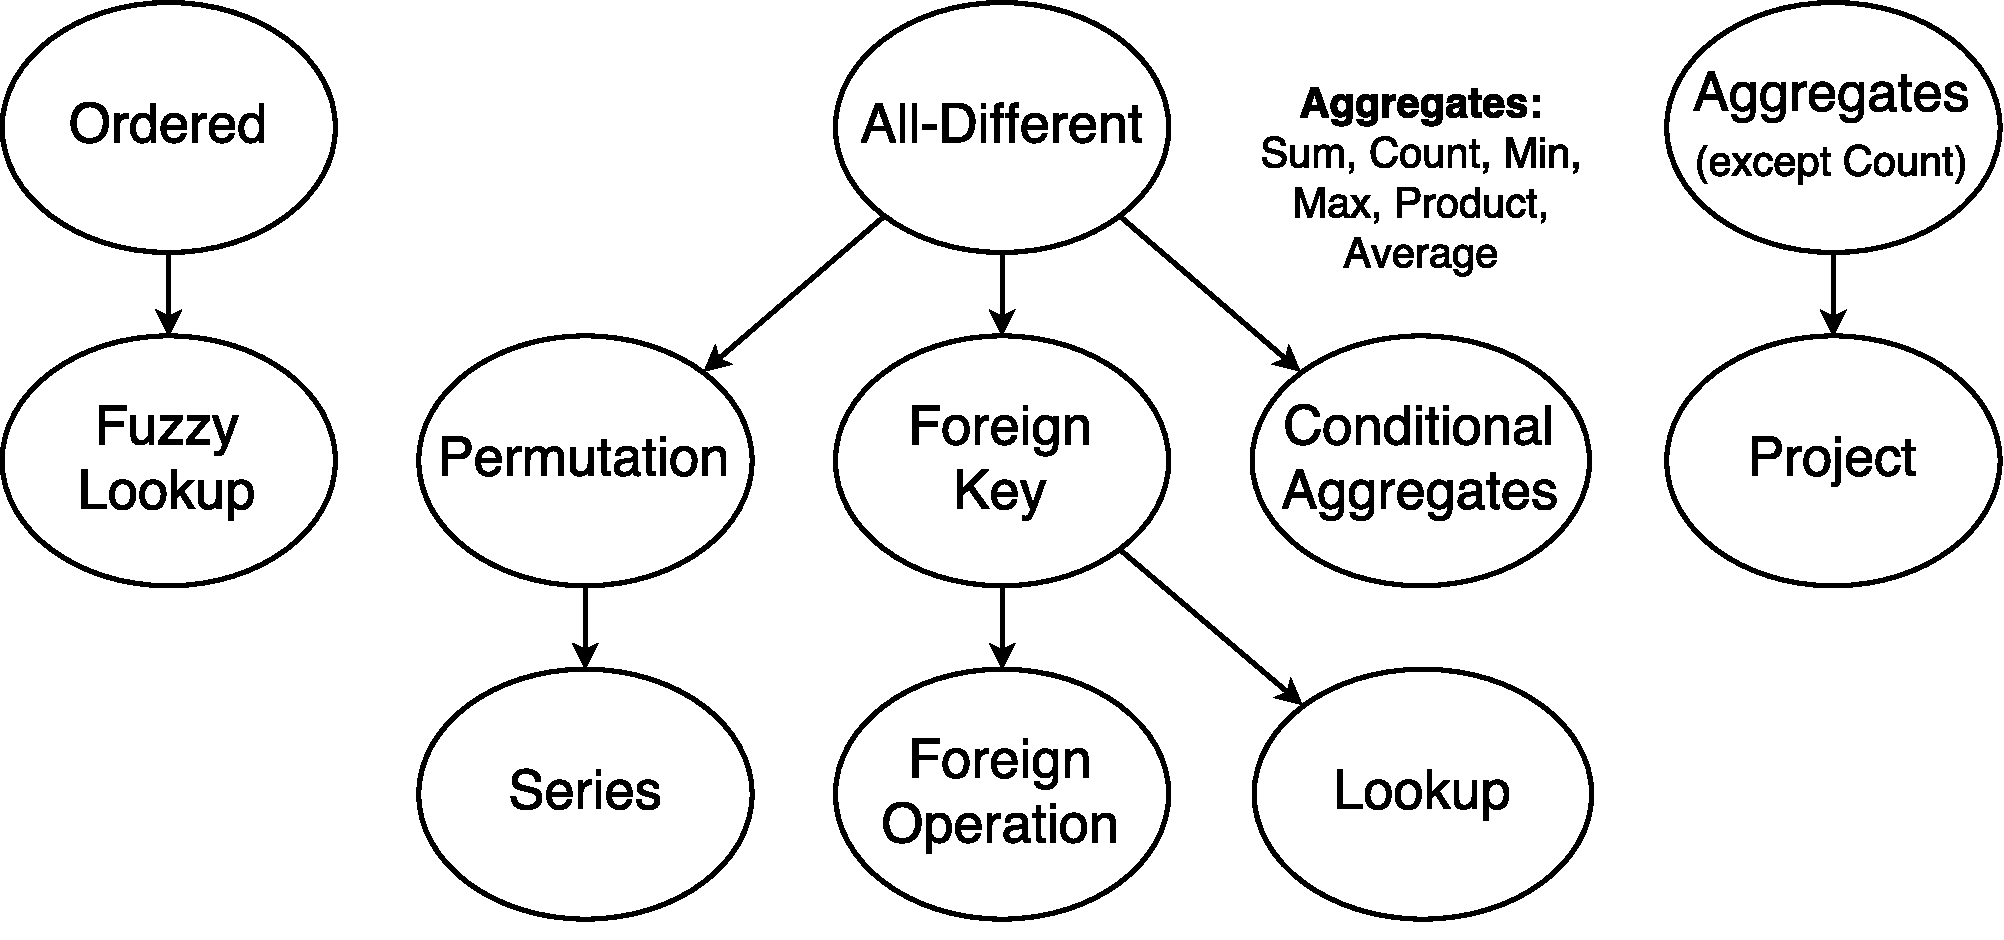
\includegraphics[width=0.60\linewidth]{constraint_dependency.pdf}
  \caption{Dependency graph of Table~\ref{table:constraints}; an arrow from~$s_1$ to~$s_2$ indicates that $s_2$ depends on~$s_1$: its signature includes $s_1$.
  }
  \label{fig:learning_order}
\end{figure}

Using the dependency graph~(\dependencies) we can reorder the templates such that a template occurs after any template it depends on.
Concretely, in Algorithm~\ref{algo:tcl} line \ref{algo:tcl:for} the input templates~$\temps$ are handled following an ordering that agrees with the partial ordering imposed by~\dependencies (e.g. \textit{ALLDIFFERENT} before \textit{FOREIGNKEY}).
When using this ordering, templates later in the ordering can use the learned constraints of the templates they depend on.
To enable this reuse of constraints, the set of learned constraints $C$ is added to the argument of \generategroups on line \ref{algo:tcl:super}.

The previously learned constraints are used to speed up the \generategroups step.
For constraint templates where some arguments are also part of a constraint that it depends on, it is not needed to search for input blocks and subblocks from scratch.
Instead, one can start from all and only the actual argument assignments of the base constraint, and only search matching input blocks for the remaining arguments.
\added{Therefore, the number of candidate assignments for a constraint template can be reduced by adding a dependence on a lower arity constraint.
}

\begin{example}
  Consider $\ecfkey{\sbl{fk}}{\sbl{pk}}$, which states that every value in $\sbl{fk}$ also exists in $\sbl{pk}$; its signature includes $\ecalldiff{\sbl{pk}}$. There are 18 \textit{ALLDIFFERENT} constraints to be found in Figure~\ref{fig:main_example}, hence, the \generategroups only needs to check which input blocks for $\sbl{fk}$ are compatible (different table, same type) with these 18 assignments to $\sbl{pk}$.
\end{example}

In this case, instead of generating one CSP to find all assignments, a CSP is generated for every known assignment of the depending constraint, which then searches for all assignments completing this partial assignment.
The procedure to generate CSPs remains the same otherwise.





\subsubsection{Redundancy}
We consider two types of redundancy that we aim to eliminate during search.
\added{Specifically, these redundancies are taken into account in the implementation for finding subassignments for a constraint.}
As noted in Section~\ref{sec:form:dependencies}, for some constraint templates there are \textit{symmetries} over the arguments that lead to trivially equivalent solutions, for example, $\ecprod{\sbl{3}'}{\sbl{1}'}{\sbl{2}'} \Leftrightarrow \ecprod{\sbl{3}'}{\sbl{2}'}{\sbl{1}'}$.
Such duplicates are avoided by defining a \textit{canonical} form for these constraints.
In practice, we define an arbitrary but fixed block ordering and require those blocks that are interchangeable to adhere to this ordering.
Moreover, among the semantically equivalent constraints product (\ecprod{\sbl{3}'}{\sbl{1}'}{\sbl{2}'}) and division (\eccalc{\sbl{1}'}{\sbl{3}' / \sbl{2}'}) we only added product, as well as only difference (\ecdiff{\sbl{3}}{\sbl{1}}{\sbl{2}}) and not sum (\eccalc{\sbl{1}}{\sbl{3} + \sbl{2}}). However, division and sum could easily be added, and they could equivalently be added in post-processing based on the matching product and difference constraints.


A last type of redundancy we chose to avoid during search is that there may be multiple \textit{overlapping} subblocks that satisfy the definition of a constraint template.
For example, consider the constraint $\ecsumc{\sbl{2}}{\range{T}{\rangeall}{\rangeto{1}{n}}}$ where $\range{T}{\rangeall}{\rangeto{k}{n}}$ consists of only zeros, then $\ecsumc{\sbl{2}}{\range{T}{\rangeall}{\rangeto{1}{j}}}$ will be true for all $k - 1 \leq j \leq n$.
In \sname we have, therefore, chosen to only consider \textit{maximal} subblocks.
\added{This can be seen as a bias of our system.}

In some cases a maximal subblock might falsely include irrelevant columns.
Consider input block $\bsbl{1} = \range{T}{\rangeall}{\rangeto{1}{3}} = [[200, 300], [200, 150], [1, 2]]$ and $\sbl{2} = [200, 300]$, then \sname will find the constraint $\eccalc{\sbl{2}}{\textit{MAX}(\range{T}{\rangeall}{\rangeto{1}{3}})}$.
Should the target constraint be $\eccalc{\sbl{2}}{\textit{MAX}(\range{T}{\rangeall}{\rangeto{1}{2}})}$, then \sname is only able to find exactly that constraint if $\range{T}{\rangeall}{3}$ is split off into a separate block in the block detection phase \added{or by post-processing the detected constraints}.






\subsubsection{Constraints}
\label{sec:which_cons}
The 33 constraints that are currently supported in our system are shown in Table~\ref{table:constraints}.
We included most formulas that we encountered in tutorial spreadsheets including the popular \textit{SUM} and \textit{LOOKUP} constraints.\!\footnote{\href{https://support.office.com/en-us/article/Excel-functions-by-category-5F91F4E9-7B42-46D2-9BD1-63F26A86C0EB}{https://support.office.com/en-us/article/Excel-functions-by-category-5F91F4E9-7B42-46D2-9BD1-63F26A86C0EB}}
We also added four structural constraints (\textit{ALLDIFFERENT}, \textit{PERMUTATION}, \textit{\ecascname} and \textit{FOREIGNKEY}) so that they can be used in the signature of other constraint templates; they are also popular in constraint satisfaction~\cite{modelseeker}.
\added{In our current system, the signature for these structural constraints was chosen to be \emph{strict}, i.e. only support those types that are required by depending constraints.
Therefore, \textit{ALLDIFFERENT} does not support floating point numbers and \textit{\ecascname} does not support strings.}

For \textit{LOOKUP}, aggregate constraints and \textit{PROJECT} we use optimized implementations to find subassignments instead of generic generate-and-test.

Given an input block assignment, the implementation for \eclookup{\sbl{2}}{\sbl{fk}}{\sbl{pk}}{\sbl{1}} first generates candidate vectors for \sbl{pk} and \sbl{1}, then populates a hash table that allows it to quickly look up keys, afterwards it generates candidate vectors for the remaining arguments and, finally, checks which subassignments are valid.

For aggregates (e.g. \textit{SUM}) and \textit{PROJECT}, a custom implementation is used that tries to find maximal subblocks that satisfy the constraint templates.
Instead of generating all possible subblocks, given an inputblock assignment, these implementations start from an input block and repeatedly generate and test smaller subblocks.
Therefore, once a match is found, all smaller subblocks do not need to be considered anymore.

Finally, for \textit{FOREIGNKEY} and conditional aggregates, generate-and-test is used, but in combination with caches that store intermediate results and a preparation step to populate some of the caches.
For example, for conditional aggregates, input block assignments are analyzed to find vectors with overlapping values.
These results are then cached and used to quickly reject subassignments where there is no overlap between \sbl{pk} and \sbl{fk}.

\subsubsection{Limited precision}
\added{One of the challenges of discovering mathematical functional constraints, such as \emph{product}, is that values in spreadsheets often have limited precision and might have been rounded.
Testing whether such a constraint holds for a given subassignment, e.g., \ecprod{\sbl{3}}{\sbl{1}}{\sbl{2}}, can be done by calculating the \emph{expected} result ($\sbl{1} \times \sbl{2}$) first and testing if it corresponds to the actual result ($\sbl{3}$).
For the values $\sbl{1} = [1.7], \sbl{2} = [1.8], \sbl{3} = [3.1]$, we would compute first $\sbl{1} \times \sbl{2} = [3.06]$ and conclude $[3.06] \neq [3.1]$ unless the expected result is first rounded.
Therefore, \sname analyzes how long the fractional part of an actual result is and rounds the expected result accordingly.}




\newcommand{\runtotal}{16.12}
\newcommand{\runtotalstd}{0.62}

\newcommand{\runfile}{0.50}
\newcommand{\runfilestd}{0.02}

\newcommand{\benchsize}{??}
\newcommand{\timeout}{200}

\section{Evaluation}\label{sec:evaluation}
In this section we experimentally validate our approach.
We first explain the experimental setup and illustrate it on the example in Figure~\ref{fig:main_example}, we then investigate the effectiveness of our method on synthetic spreadsheets, after which we evaluate our method on spreadsheets from various sources.

\subsection{Experimental setup}
\label{sec:evalualtion:method}
All spreadsheets used in the experiments are in CSV format and for each spreadsheet the tables are specified.
The tables were obtained by running the table extraction tool, \added{\ecautoextract}.
Manual intervention of the simple automatic detection was needed only in the case of \textit{None} values (e.g. to merge split-up tables caused by the \textit{None}'s) and in cases where the headers are ambiguous (e.g. headers containing textual and numeric cells).
In these cases the tables specifications were generated using the \added{\ecvisualextract{}} tool.

%(using a combination of the rather primitive automatic detection + visual verification that the tables are meaningful (e.g. merge split-up tables because of None values, or remove headers of all-textual tables).
%{Should we not say just with the visual tool?} {Rewrote a bit, I like the amount of detail as it provides insight into the limitations}
Blocks are then detected automatically using the block detection algorithm, \added{\ecblockdetect}.
Manual intervention was required for tables that contain \textit{None} values (e.g. if the type of empty cells cannot be inferred).

% Group definitions are only specified if the spreadsheet contains ambiguous \textit{None} values. \{What does this mean, 'group definitons'?? Is this 'block detection' (Sec 4.2), if so, how do we explain this process??} 

All spreadsheets also have a set of ground-truth of constraints, we call these the \textbf{intended} constraints, that are expected to be (re-)discovered.
These were determined by us using either the formulas of the original sheet if present, or inferring them based on, for example, the header names in the sheet.
Five spreadsheets contained rows or columns that were entirely identical in which case results can be computed in multiple ways and there are multiple valid constraints.
\added{For these spreadsheets, we used the original formulas when present and otherwise inferred the intended constraints based on the headers and the location within the sheet. However, some of the intended constraints are currently outside of the scope of \sname, in particular nested mathematical or nested logical formulas. We denote by \textbf{supported} constraints the subset of intended constraints that the system can find in theory.

%Section~\ref{sec:which_cons} discusses the 33 constraints currently supported by \sname.
In the following experiments, we focus on spreadsheets specifically and hence only include \textit{functional} constraints, constraints that can be expressed as formulas.
Therefore, we filter out the structural constraints \textit{ALLDIFFERENT}, \textit{FOREIGNKEY}, \textit{PERMUTATION} and \textit{\ecascname} in the output.}
%
%and any intended constraint involving one such vector was also added for the equivalent vectors. \{They are usually not copied} 
%
All constraints are stored in their canonical form.

We will use recall and precision to measure how well our tool is performing. Recall is the fraction of intended constraints actually discovered by the system: $\frac{\text{intended discovered}}{\text{all intended}}$, while precision is the fraction of constraints found by the system that are indeed intended: $\frac{\text{intended discovered}}{\text{all discovered}}$.

\added{We include a \emph{no-CSP} baseline to compare our approach to.
This baseline follows a similar approach as \sname, however, it does not prune input blocks in step~3a and generates subassignments directly.
Therefore, the signature is also only tested on the subassignment level.
While the modified approach still benefits from the reuse of earlier solutions, it does not generate partial assignments for dependent constraint templates.
}

All experiments were run using Python 3.5.1 on a Macbook Pro, Intel Core i7 2.3~GHz with 16GB RAM.
The constraint solver that is used by the input block assignment phase (Step 3a) is python-constraint \cite{python_constraint}.



\subsection{Results on the running example}
For the example presented in Figure~\ref{fig:main_example},
\sname takes a few seconds to find the constraints listed in Figure~\ref{fig:sol_example}.
These include 5 spurious $\textit{RANK}$ constraints, e.g. $\ecrank{\range{T_1}{\rangeall}{1}}{\range{T_1}{\rangeall}{5}}$, that are true by accident.
Moreover, there is one \textit{LOOKUP} constraint that was not intended in the original spreadsheet (looking up ID based on Salesperson) and which is symmetric to the intended one (Salesperson based on ID).

Hence, for this example we achieve a recall of 100\%, that is, all intended constraints are discovered, and a precision of $12/18 = 67\%$. All intended constraints are supported. The recall is perfect, but the precision is rather low. This is mostly due to the spurious RANK constraints. We note that the tables are quite short, which increases the chance of a constraint like \textit{RANK} to be true by chance; we expect less spurious constraints on larger datasets.

We now investigate three main questions that influence the quality of the solutions found by a constraint learning method:
\begin{itemize}
\item \textit{\qone}: the method may fail to find intended constraints if it takes too much time to find them; what are the factors that influence the runtime of the method most?
\item \textit{\qtwo}: the method may fail to find intended constraints because it does not support such constraints; how does our method perform on real spreadsheets?
\item \textit{\qthree}: the method may find non-intended constraints; how many and what type of non-intended constraints are found on real spreadsheets?
\end{itemize}
We first investigate \textit{\qone} on synthetic spreadsheets and investigate \textit{\qone}, \textit{\qtwo} and \textit{\qthree} on a collection of real spreadsheets.


\subsection{Effectiveness on synthetic data}

\begin{figure}[t]
  \centering
  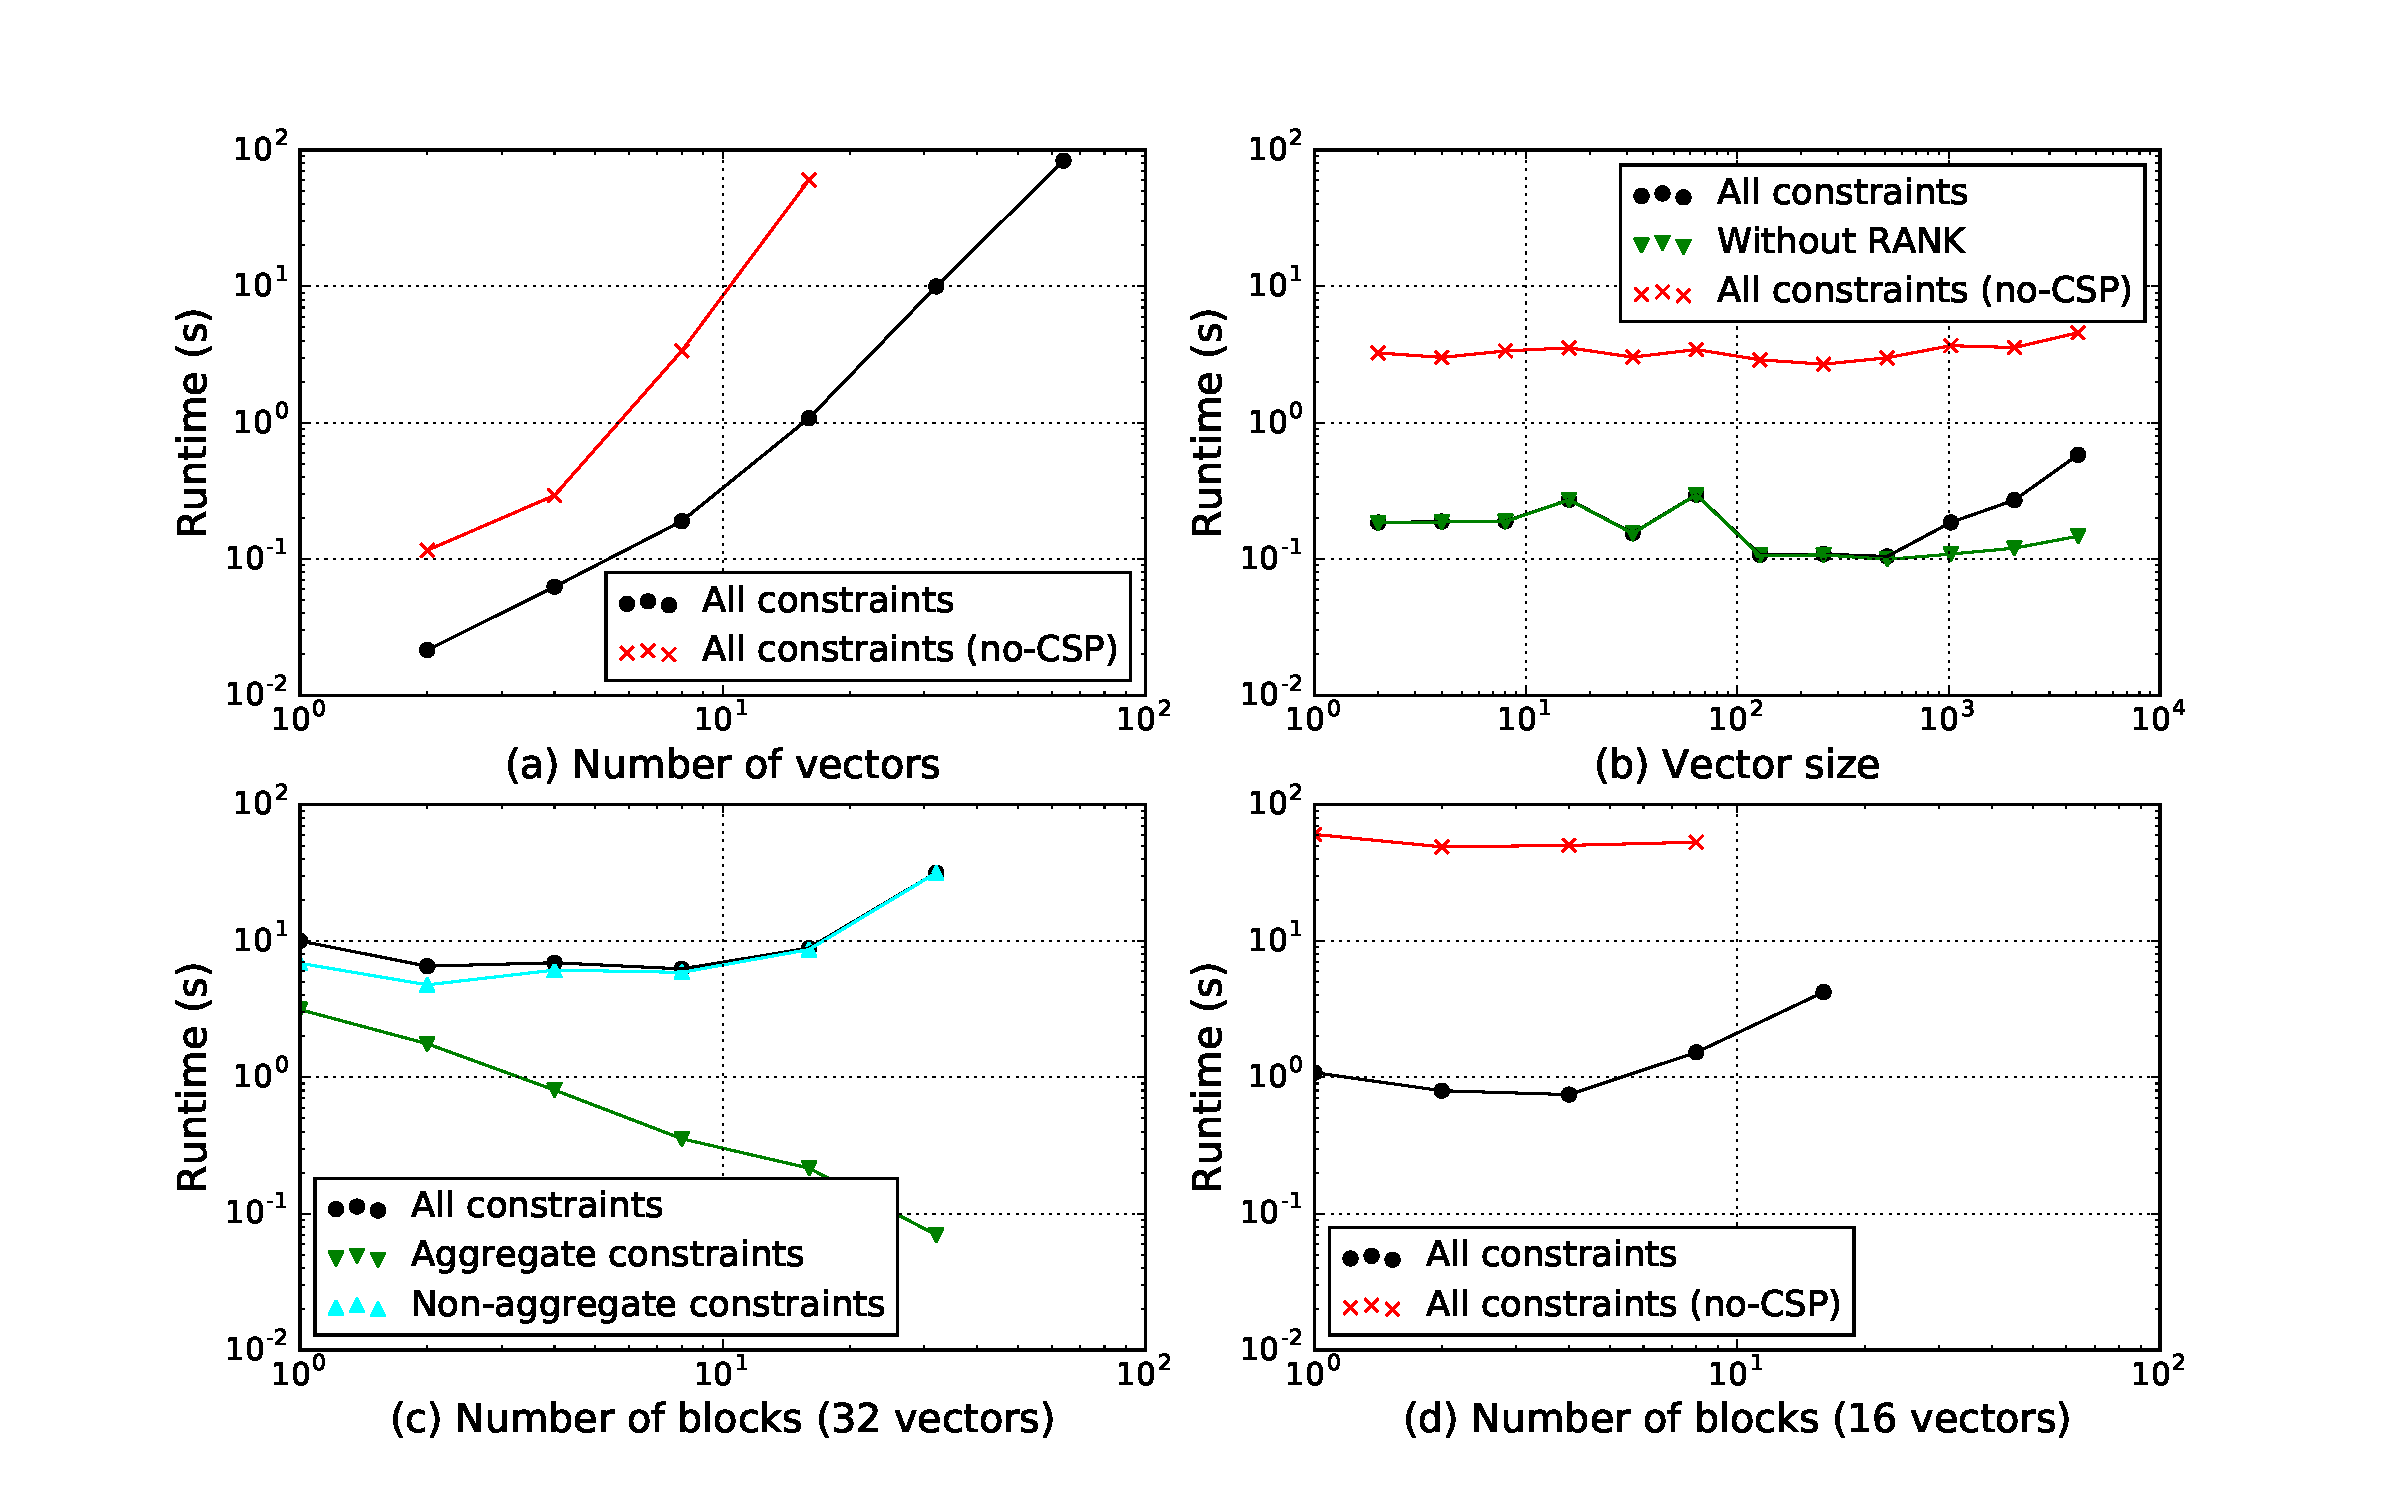
\includegraphics[width=\linewidth]{scatter_plots.pdf}
  \caption{Loglog plots of the experiments with synthetic (random) data. In plot~$a$ the number of vectors is increased; in plot~$b$ the size of the vectors is increased; and in plots~$c$ and~$d$ the number of blocks is increased (the block size is decreased).
  \added{Missing values for the no-CSP baseline indicate that it timed out.}}
  \label{fig:runtime_analysis}
\end{figure}


In this section we investigate the factors that influence the runtime of \sname the most; we do this by investigating the impact on the running time of 1)~the number of vectors; 2)~the length of the vectors; and 3)~the size of the blocks.
This analysis is accomplished by testing our system on synthetic spreadsheets. \added{The timeout for all experiments was set to~\timeout~seconds.}

\paragraph{Spreadsheet generation.}
%For our analysis, we perform multiple experiments on synthetically generated spreadsheets.
The synthetic sheets should trigger the checking of many different constraints, both in the first phase (input block assignment) and in the second phase (subblock assignment), in order to clearly study the effect on the constraint checking. As many constraints require numeric or discrete data, we will use integers in the synthetic sheets as these are both numeric and discrete.

We generate spreadsheets with random data. The result is that there are no intended constraints in the data. This is reasonable, as even in real data most of the constraints will not hold. Additionally, for vectors in random data the \textit{ALLDIFFERENT} constraint is likely to hold, which is a requirement for many other constraint templates.

The synthetic spreadsheets contain two tables, because a number of constraints require that their arguments are picked from different tables. For one table the number of vectors and block size is fixed to two, while for the other table these properties are varied according to the experimental setup.
The reported number of vectors and the block size in the experiments refer to those of the second table. The length of the vectors can also be adapted and applies to both tables, since equal length vectors are a required property of many constraints.
Unless otherwise mentioned, the 'adaptable' table consists of one block of $8$ vectors of length $8$, and hence 2 vectors of length $8$ in the 'fixed' table.
%The running times for various configurations are plotted in Figure~\ref{fig:runtime_analysis}. % no such general pointer, specific pointers only


%Recall that our method uses a 2-phase approach where in the first phase, the superblock assignments are generated (Section~\ref{sec:algo:super} and in the second phase, the subblock assignments are generated (Section~\ref{sec:algo:subgr}).

\paragraph{Effect of number of vectors}
Figure~\ref{fig:runtime_analysis} (a) shows the results of our experiments, in which \sname was run on synthetic spreadsheets containing an increasing number of equally sized vectors.
As shown in the figure, the number of vectors in a spreadsheet can have a significant impact on the running time.
\added{Moreover, \sname performs favorably to the no-CSP baseline whose running time not only starts off slower but also grows faster.}

The number of vectors is expected to impact the running times, especially when few input block assignments can be discarded in the first phase.
This occurs, for example, when most vectors belong to the same block or all vectors have the same type and size as we artificially enforced in this experiment.
In this case, for a constraint template that requires $n$~single vector arguments and a spreadsheet with $v$~vectors, up to $\frac{v!}{(v - n)!}$ subassignments are generated and checked by the algorithm.

Typically, we expect the number of generated subassignments to be much smaller in real world spreadsheets and, therefore, the running time to be less sensitive to the number of vectors.
This is because in the first phase entire blocks can be disqualified that do not match the signature requirements, e.g. blocks of vectors with different lengths. % for the product constraint.


% Many constraints take single vector arguments, therefore, the total number of subassignments that are generated in the second phase of the algorithm depends on the number of vectors in the spreadsheet and the arity of the constraint.


% For a constraint template with arity~$n$ and $v$~vectors there are $n^v$ subassignments (or $\frac{n!}{(n - v)!}$ if the arguments have to be different). tias{Better move to 4.3.2? or have there too anyway, no new facts in 'experiment' section}
% As the number of vectors in a spreadsheet increases, the running time will quickly be dominated by constraints with a larger arity.
% This effect is noticeable in our synthetic experiments when the number of (equally sized) vectors tias{more details about equal sized: is this a strict requirement for this to happen? I assume this is worst case and does not happen that much in practice? (the next sentences half hint at that, be more explicit)} is increased (Figure~\ref{fig:runtime_analysis}a).

\paragraph{Effect of length of vectors}
%The benchmark experiments show that the number of cells in a spreadsheet has a very limited impact on the running time.
To measure the effect that the length of the vectors has on the running time, we ran our system on spreadsheets in which the length of the vectors was gradually increased.
Figure~\ref{fig:runtime_analysis} (b) summarizes our results and shows that the length of the vectors has a small impact on the performance for most templates.
\added{The no-CSP baseline performs similarly, however, its runtime is higher by a large margin.}

As discussed in Section~\ref{sec:which_cons}, our implementation attempts to detect as fast as possible if a subassignment does not satisfy a constraint template.
Our experiments satisfy the assumption that the large majority of possible subassignments do not satisfy most constraints.
Therefore, the results confirm that our implementation is able to severely limit the impact of the length of vectors.

Most of the increase in running time can be attributed to the \textit{RANK} constraint.
The implementation is often not able to quickly detect that subassignments do not satisfy \textit{RANK}, meaning that it will have to analyze many if not all entries in the vector.

\paragraph{Effect of block size}
To measure the effect of changing the block size, the number of vectors is set to~$32$ and the vectors are explicitly split into varying number of blocks/tables (up to ~$32$).
Figure~\ref{fig:runtime_analysis} (c) shows the running times of \sname for various settings.
As the blocks become smaller, the total running time first decreases before increasing again.
Looking at the running times for aggregate constraints and non-aggregate constraints  separately reveals that they are affected differently by the block size.
For aggregate constraints (green line) the running time decreases with the block size, while for non-aggregate constraints (red line) the running time first stays more or less constant but then increases more strongly as the size of the blocks becomes small.

Aggregate constraints, e.g. sum or max, have an argument that allows subblocks of varying sizes while non-aggregates only allow single vector arguments. Hence, for aggregate constraints our method will try to find any subblock in the given input block that satisfies the constraint.
Since a input block of size~$m$ has $m(m+1)/2$ contiguous subblocks, the search for aggregate constraints becomes faster if there are more but smaller blocks\footnote{Consider, for example, $v$~vectors distributed over $b$~blocks of size $v/b$, the number of subblock candidates then is $O(b * v^2 / b^2) = O(v^2 / b)$}.

Non-aggregate constraints have only single vector arguments.
%Therefore, the total number of subassignments generated by the algorithm is not influenced by the block size.
By splitting a set of vectors into many blocks, however, there will be a larger number of input blocks given as input to the first phase. 
%Recall that in phase~1 the algorithm additionally tests block level properties for every superblock assignment.
In the synthetic spreadsheets, the first phase, which looks at properties of input blocks alone, can disqualify few or no input block assignments, leading to some increase in runtime as more blocks are added.

\added{In order to compare to the baseline, we had to lower the number of vectors from~$32$ to~$16$.
Figure~\ref{fig:runtime_analysis} (d) shows that here, too, our system performs better.
Both approaches profit from lower running times for aggregates and the no-CSP baseline can offset some of the slowdown as the block size grows small.}

%therefore, it will be faster to group the same vectors into larger super blocks, generate fewer superblock assignments to test and split these into single vector subassignments in phase~2.

%tias{I'm cutting this paragraph, in an unsupervised method you do not control the number of blocks and will hence not 'split unrelated vectors'; that would be supervised.}
%Splitting unrelated vectors into smaller subblocks can decrease the running time for some spreadsheets by reducing the workload for aggregate constraints.
%However, the two phase approach is also well suited to operate on large blocks and eliminate superblock assignments that are not compatible with constraint template signatures. samuel{Does this conclusion sound sound?}

% tias{Point to figure to support this (actually, move that line into 4c??); also, if this is true, you are basically saying that the CP-based first phase is worse then the second phase? That kind-of demotivates the idea of using CP in first phase... What do you really want to share with the reader?}

$ $

\noindent 
These experiments with synthetic data have given us a better understanding of what effect the properties of vectors and blocks can have on runtime and hence on the ability of the algorithm to finish within reasonable time. We next investigate the behavior of our method on real spreadsheets.


\subsection{Effectiveness on real spreadsheets}\label{subsec:real_spreadsheet_experiments}
\added{
In order to test our approach on real data we assembled a benchmark of spreadsheets from three sources:
1)~spreadsheets from an exercise session for teaching Excel at the Brussels Business School based on the book~\cite{excel_book}, covering the most popular Excel formulas; 2)~spreadsheets from online tutorials on Excel formulas; and 3)~publicly available \textit{data} spreadsheets such as real-world crime statistics (FBI:UCR) or financial reports (US BEA). The data and its extended description are available in Appendix \ref{appendix:dataset_overview} in Table \ref{tab:constraint_by_category} and at the same repository as before with the links to all original publicly available spreadsheets used in the experiments.
} 


Table~\ref{tbl:category_overview} gives an overview of the spreadsheets in the different categories and summarizes the results of our experiments.
The data is also visualized in Figure~\ref{fig:comparison}.


{\setlength{\tabcolsep}{0.33em}
\begin{table}[htb]
  \centering
  \caption{Summary of properties and results per spreadsheet category}
  \label{tbl:category_overview}
  \begin{tabular}{lccccccc}
 & \multicolumn{2}{c}{\textbf{Exercises} (9)} & \multicolumn{2}{c}{\textbf{Tutorials} (21)} & \multicolumn{2}{c}{\textbf{Data} (4)} \\
 & Overall & Sheet avg & Overall & Sheet avg & Overall & Sheet avg \\ \hline
    \textbf{Tables} & 19 & 2.11 & 48 & 2.29 & 4 & 1 \\ \hline
    \textbf{Cells} & 1231 & 137 & 1889 & 90 & 2320 & 580 \\ \hline
    \textbf{Intended constraints} & 34 & 3.78 & 52 & 2.48 & 6 & 1.50 \\ \hline \hline
\textbf{Recall (all)} & 0.88 & 0.85 & 0.88 & 0.87 & 1.00 & 1.00 \\ \hline
\textbf{Recall (supported)} & 1.00 & 1.00 & 1.00 & 1.00 & 1.00 & 1.00 \\ \hline
\textbf{Precision} & 0.94 & 0.96 & 0.69 & 0.90 & 1.00 & 1.00 \\ \hline
\textbf{Runtime \sname} & 0.91 & 0.10 & 0.87 & 0.04 & 0.79 & 0.20 \\ \hline
\makecell{\textbf{Runtime no-CSP}\\\textbf{baseline}} & 58.36 & 6.48 & 36.84 & 1.75 & 19.73 & 4.93 \\

\end{tabular}
\end{table}}

\paragraph{\qone: Effectiveness}
Our first question, \qone, is about the inability to find intended constraints due to excessive runtime. As Table~\ref{tbl:category_overview} (last row) shows, the runtime of our method on these spreadsheets is always fast.  
The average runtime across all spreadsheets is $0.08s$.
Across categories the average running times fluctuate in the range between $0.04s$ to $0.20s$.
While most spreadsheets can be processed very quickly, running times can go up to around $0.61s$ for others.
In the previous section we analyzed the effect of various factors that can help explain runtime behavior on data generated to allow many candidate subassignments (e.g. using only vectors of the same type and length).
Our benchmark experiments show that our algorithm is able to perform well on real spreadsheets, even for larger numbers of vectors.
\added{Moreover, these experiments validate our two-step approach, since \sname is able to find constraints 20 to 60 times faster than the no-CSP baseline.}

% Most of the execution time in these cases goes towards searching either aggregate constraints or conditional aggregates.
% The search for aggregates will be slow on spreadsheets containing larger groups of numeric data.
% For conditional aggregates the number of candidate primary keys (all-different) and numeric vectors determines the running time (e.g. the case study example).


%We explained various optimizations, most notably the exploitation of dependencies.
%Using the dependencies to find constraints incrementally cuts down large parts of the search trees, especially for constraints that have many arguments.
%Essentially, one obtains a more specialized search without much effort.

Looking at the runtime per constraint template individually, the slowest by far is fuzzy lookup using $\pm 21\%$ of the running time.
It is followed by product ($\pm 7\%$), relative difference ($\pm 6\%$), running total ($\pm 5\%$), difference ($\pm 5\%$) and various row-aggregates ($\pm 5\%$).

\added{Dependencies are optional and do not affect precision or recall.
However, our method can exploit dependencies in order to find constraints incrementally and increase the systems efficiency.}
To illustrate the effect this can have, we ran the benchmarks without using \textit{\ecascname} as base constraint for fuzzy lookup.
The total running times per category increase by 74\% (exercises), 84\% (tutorials) and~13\% (data).
\added{This shows that the use of dependencies can have a strong effect on running times by reducing the number of candidate assignments for depending constraints and sharing the computation and pruning done for one constraint with another.}
 % (0.83 + 1.03 + 0.99) = 2.85 / (1.34 + 1.46 + 0.46) = 3.3  / (0.99 + 0.98 + 0.44) = 2.41


\begin{figure}[t]
  \centering
  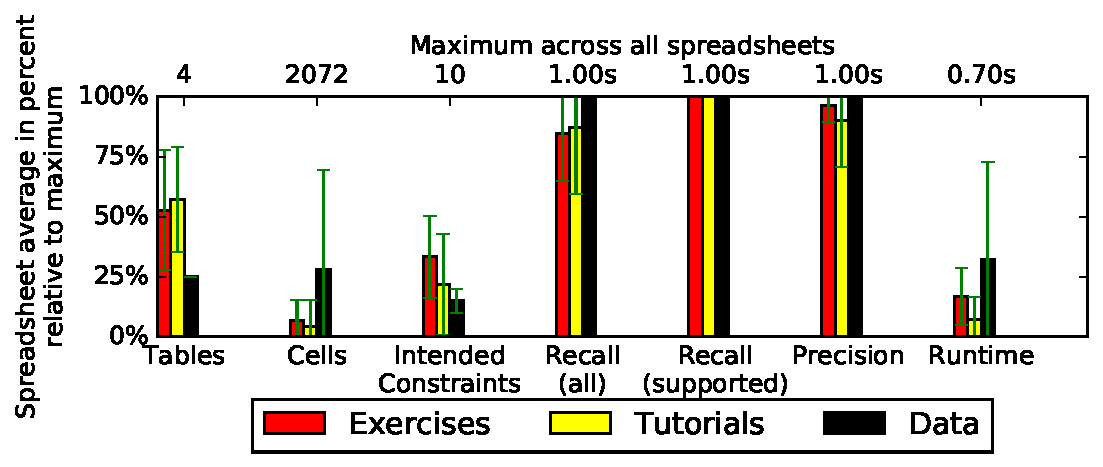
\includegraphics[width=1\linewidth]{comparison.pdf}
  \caption{\added{This figure visualizes the data from Table~\ref{tbl:category_overview}, i.e., the average properties and performance of spreadsheets within every benchmark category.
  Values are scaled relatively to the \emph{maximum value across all individual spreadsheets}}.
  Green bars indicate standard deviation within the category.}
  \label{fig:comparison}
\end{figure}


\paragraph{\qtwo: Intended and supported constraints}
The overall recall achieved by our system, \sname, is~$0.88~(81/92)$.
When looking at the recall per category, \sname is able to consistently obtain high values for both overall and average recall, as shown in Table~\ref{tbl:category_overview}.
The intended constraints not discovered correspond to constraints that are not supported by the system, hence the supported recall is 1.
Therefore, \sname is able to find all constraints for supported constraint templates, which shows that our method is able to learn all constraints using the bias chosen, that is, the formalism of signature and definition. 

% The intended constraints not discovered correspond to constraints that are not supported by the system (supported recall is 0.99), except for one intended \textit{SUMIF} constraint.
% The supported recall value mostly confirms that our bias (signature) is not too restrictive and is able to find constraints for supported constraint templates.
% By changing the signature of \textit{SUMIF} to allow \sbl{pk}

The intended constraints that are not discovered correspond with nested constraints (e.g., $R = \frac{W}{(L/100)^2}$), variants of supported constraints (e.g., series that do not start at 1) or more complex versions of supported constraints (e.g. conditional aggregates whose conditions are constant values). 

\paragraph{\qthree: Precision}
%\item \qthree: it may find non-intended constraints; how many and what type of non-intended constraints are found on real spreadsheets?
The final question, \qthree, is about the amount and type of \textbf{non}-intended constraints found.
Across all spreadsheets \sname achieves a precision of~$0.79~(81/103)$.
While the average precision per spreadsheet is high, over $0.90$ in every category, we observe that the overall precision is much higher for the exercises and data categories ($0.94$ and $1.00$) than for the tutorials category ($0.69$).

Examining the tutorial spreadsheets confirms that there are a few spreadsheets that have a high number of additional constraints, e.g., one spreadsheet computes aggregates on inventory data, but copies the data column for every aggregate.
Since every aggregate can be calculated based on any of the equal columns, our method will find all of these constraints.
However, for every aggregate only one constraint is considered to be \textit{intended}, the others will be considered as redundant and decrease the precision.

%many of the resulting constraints will be marked as unintended. tias{rewrite 'many of the..' into 'our method will find all of these; only one in 'true' set, others drive down precision...'}

Such redundant or unintended constraints are the result of multiple ways to calculate the same result, e.g., if there is duplicate data as in the example above.
One way to increase precision for this case is to post-process the constraints to detect equivalences and implications, and heuristically select one among multiple ways to compute the same vector.





%\subsection{Testing the limits}
%Our algorithm relies on a correct table and group detection step, and we noticed that exported CSV files can make this more difficult in case of rounding errors due to low-precision formatting as well as misformatting of strings so they are interpreted as numbers.
%Automatically generated sheets can also contain many duplicate (equal) rows or columns, which are a source of increased runtime and decreased recall for our algorithm. For example, we tested a spreadsheet (``exps'') with 6~tables, 531~cells and many duplicate columns across tables.
%While we obtained a recall of~$1.0$, the algorithm ran for $14.30s$ and the overall precision was~$0.52$ and only~$0.11$ when counting constraints with equal columns separately.
%%By using a (heuristic) post-processing step the precision for this example could be increased.
%%The running time can be improved by implementing additional optimizations.




\section{Applications}\label{sec:applications}
\added{In this section, we illustrate how two of the motivating applications, auto-completion and error checking, can build on our method for solving the tabular constraint learning problem.}





\subsection{Auto-completion}
Auto-completion can be seen as using knowledge derived from the current data to predict new values before they are written by the user.
\added{
We can decompose this process into three phases: 1) learn constraints on a snapshot of the spreadsheet; 2) new data~($\Delta D$) is added by the user; and 3) the system uses the learned constraints to predict missing values.

Step~1 corresponds to running \sname on the snapshot to discover constraints in the spreadsheet.
In step~2, the user extends one or more vectors in the spreadsheet with new values.
These extended vectors now stretch beyond the original table they are situated in.
Therefore, the remaining vectors and blocks in the same table are marked as \emph{incomplete}, indicating they are missing some values required to complete the table.
Finally, in step~3, \emph{functional} constraints discovered in step~1, are used to predict missing values.
A functional constraint, such as $\ecsumc{\sbl{r}}{\mathbf{\sbl{x}}}$, calculates a result~($\sbl{r}$) based on its \textit{input}~($\mathbf{\sbl{x}}$).
Hence, a functional constraint can predict missing values if the result block is incomplete and none of the input blocks is incomplete.


%A snapshot~($D_0$) is used to learn constraints and these are combined with new data~($\Delta D$) that the user has added.
%Using~$\Delta D$ we can keep track of which vectors have changed and which vectors are now \textit{incomplete}.
%\textit{Functional} constraints, such as $\ecsumc{\sbl{r}}{\mathbf{\sbl{x}}}$, are able to compute a result~($\sbl{r}$) based on its \textit{input}~($\mathbf{\sbl{x}}$).
%If all vectors in the input blocks have changed and the result vector is incomplete, the constraint can compute the resulting value(s).

Let us illustrate this application on the two-table spreadsheet shown in Figure~\ref{fig:autocompletion_example}.
First, we run \sname on tables~$T_1$ and~$T_2$ (in green) and discover the constraints $\ecsumif{\range{T_2}{\rangeall}{2}}{\range{T_1}{\rangeall}{2}}{\range{T_2}{\rangeall}{1}}{\range{T_1}{\rangeall}{3}}$ and $\ecsumif{\range{T_2}{\rangeall}{3}}{\range{T_1}{\rangeall}{2}}{\range{T_2}{\rangeall}{1}}{\range{T_1}{\rangeall}{4}}$.
Afterwards, vector~$\range{T_2}{:}{1}$ is extended with a new value \textit{West} and vectors~$\range{T_2}{:}{2}$ and $\range{T_2}{:}{3}$ are marked as incomplete.
Finally, the \textit{SUMIF} constraints are used to complete their incomplete result blocks, suggesting $\range{T_2}{4}{2} = 1547$ and $\range{T_2}{4}{3} = 428128$.

In an interactive setting, auto-completion can be performed whenever new values are entered, however, to update the learned constraints, \sname would need to consider only assignments containing modified vectors.
}

%In case multiple constraints predict different values for the same cell, the algorithm will have to either prioritize constraints based on their specificity or a heuristic, not make a prediction, or present the choice to the user.

\subsection{Error detection}
\begin{figure}[t]
% %\begin{subfigure}{.70\textwidth}
%   \begin{center}
%     \includegraphics[width=\width]{figures/fbi_figure_highlighted.png}
%   \end{center}
%   \caption{Real world tabular constraint reconstruction: FBI crime statistics}
%   \label{fig:fbi}
%\end{subfigure}
% \hfill
% \begin{subfigure}{.29\textwidth}
\begin{center}
    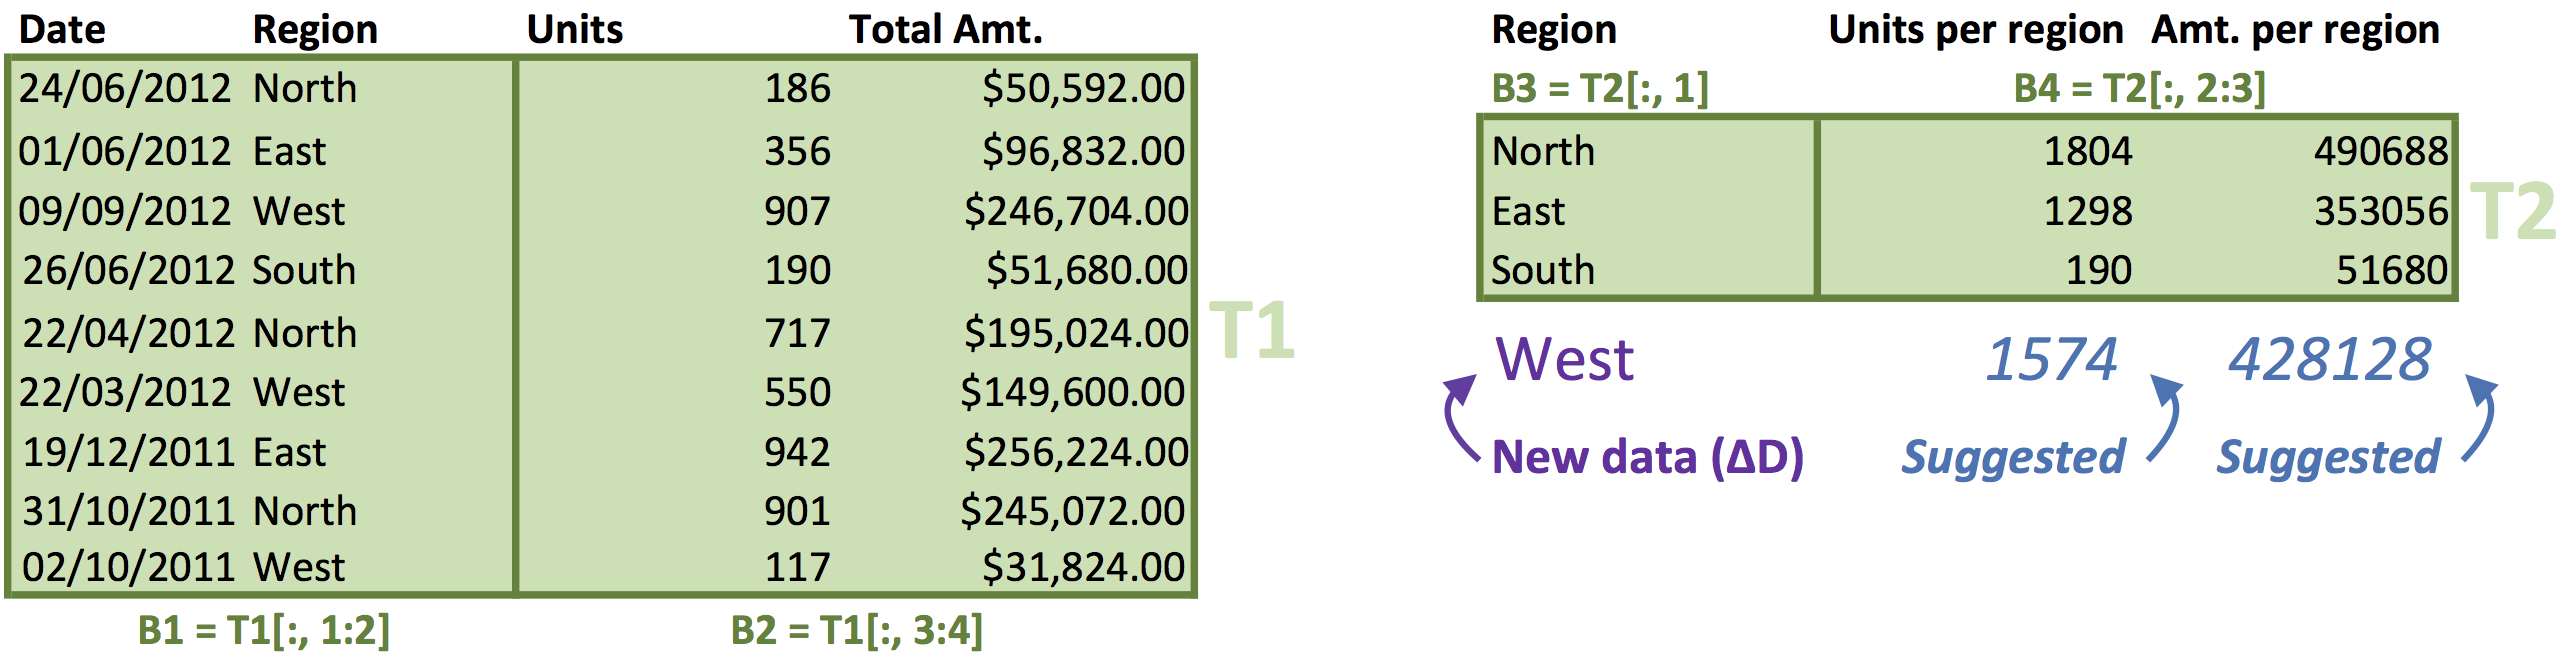
\includegraphics[width=1.0\linewidth]{Learning3.png}
  \end{center}
  \caption{Auto-completion works by learning constraint on a snapshot \added{(green tables~$T_1$ and~$T_2$)} and combining those constraints with new data $\Delta D$ \added{(purple)}.
  \added{For example, in this figure a user types a new value \textit{West}. The system can then suggest values (blue) for the other cells in that row.}}
  \label{fig:autocompletion_example}
%\end{subfigure}
\end{figure}


We discuss two cases of error detection.
The first setting is the \textit{online} detection of errors and is similar to the auto-completion setting.
\added{Constraints are learned on a snapshot before new data is added.
Functional constraints whose result block was modified are checked on the new data.
If such a constraint does not hold anymore, it could indicate errors such as typing errors in the data just entered.
For example, filling in $\range{T_2}{4}{2}=1572$ in Figure~\ref{fig:autocompletion_example} would violate the corresponding \textit{SUMIF} constraint and likely indicate an error.}

% If a constraint does not hold anymore on the new or modified data}
% Using snapshots, one can learn the constraints in the previous snapshot and search for \textit{conflict} constraints, which do not agree with newly added data~$\Delta D$.
% Such conflicts can indicate (typing) errors in the data just entered. For example, in case $1572$ was added in Figure~\ref{fig:autocompletion_example} for \textit{Units per region} in the newly added row (\textit{West}).

%Conflict constraints can indicate errors in the input.
%However, such conflicts can be wrongly caused by spurious constraints.
%Hence, conflicts should perhaps only be detected if the snapshot data is large enough.
%An exact specification of what large enough means (i.e., how to measure the confidence in the constraint violation) is a separate application-dependent research question and will be investigated in the future work.
\added{The second setting is \textit{offline} error detection, that is, on a given file.
% Consider a use case concerning crime statistics provided by the FBI in Figure~\ref{fig:fbi}.
% Our system is able to detect the second sum constraint, however, a missing value prevents the first sum constraint from being learned.
% A possible approach to detect such missing or wrong values is to look at a sample of the table, e.g. trying to leave out each row, and compare the constraints learned on this sample with the constraints learned on the whole table.
  %The sample needs to be large enough such that we have enough confidence that the constraints are correct. For example, in Figure \ref{fig:fbi} all but one row satisfy the constraint, which is a strong indication that there is a constraint violation.
First, \sname is run to detect all constraints~($S$) in the given spreadsheet.
Then, from this spreadsheet, one can repeatedly remove one or multiple rows or columns~($v$) and detect all constraints~($S_v$) that hold in the modified spreadsheet.
Every constraint in $S_v$ that did not occur in $S$ is violated by a value in the rows or columns~$v$ that were removed.
Therefore, values in the rows or columns~$v$ that occur in such a violated constraint can be marked as potential errors to be reviewed by a user.
This approach allows constraint discovery to be treated as a black-box, however, it requires a scheme for choosing which row(s) or column(s) are removed.

Alternatively, we propose to extend current constraint definitions to tolerate up to a given number of wrong values and report these.
This approach would be more robust, however, it requires definition tests to be able to deal with wrong values.}


% between the original spreadsheet and a sheet with a row or column removed. Many schemes can be devised for choosing which row(s) or column(s) are removed. tias{Expand 'one can repeatedly search' into the actual steps: take spreadsheet, remove row/column, detect constraints and then search for any constraints not present in the full data (can easily be optimized to avoid known constraints btw)}
%This task can be formulated as online error detection by repeatedly partitioning the spreadsheet into a snapshot~$D_i$ and ``input'' $\Delta D_i$ (e.g. leave out each row and consider it as $\Delta D_i$) to detect conflicts.

%Of course, generating large enough samples and rows (columns) to be added can be done in multiple ways.
%In the limited case of detecting single errors one can leave out every row (column), consider the remaining data to be the sample and
%and the left out row (column) to be new input.

\section{Conclusions}\label{sec:tacle_conclusions}

% points: 1) can be a base for an actual plugin or a function in excel 2) novel problem and challenge for systems and constraint solvers 3) can be part of the complicated pipeline togehter with the header detection
Our goal is to automatically identify constraints in a spreadsheet.
We have presented and evaluated our approach, implemented as the system \sname, that is able to learn many different constraints in tabular data.
The resulting method has high recall, produces a limited number of redundant constraints and is sufficiently efficient for normal and interactive use.
Our approach also allows new constraint templates to be easily added by specifying their signature in terms of properties and providing an implementation that finds subassignments satisfying the definition.

The approach is designed to find constraints that hold over entire columns and rows. In future work we plan to extend this to learn arbitrary nested constraints (e.g. $\sbl{4} = (\sbl{1} + \sbl{2}) / \sbl{3}$), as well as constraints over only a subset of the vectors. This may give rise to more redundant and spurious constraints, which was not problematic up to this point.

Two promising ways to mitigate redundant and spurious constraints are heuristic filtering or post-processing of the constraint set and the integration of our approach in an interactive setting where users can receive and provide feedback.
The latter is more similar to an active learning setting.

\added{A final direction is that the current approach assumes consistent (noise-free) data, typically generated by some external system. We do support the detection of limited precision calculations as this is a type of noise generated by exporting data. Also, our approach can be used for error correction in case some noise/errors are assumed. However, in inductive logic programming there has been much work on how to handle constraints over noisy data such as allowing a tolerance level $\epsilon$ when a rule or a constraint $\sum_{i=1}^n b_i = c$ matches up to $\epsilon$: $|\sum_{i=1}^n b_i - c| \leq \epsilon$, while in constraint satisfaction a popular alternative is to consider \textit{soft} constraints that can be violated at a cost, which is a real value, and then the task is to find the top-$k$ best matching constraints.
Threshold bounded error tolerance can be supported by adapting constraint definitions to allow such noise.}
This could extend the approach to new application domains, beyond traditional spreadsheets.


\section{Spreadsheet Dataset Overview} \label{appendix:dataset_overview}
\added{
We collected spreadsheets from three main sources.
\begin{itemize}
  \item After identifying popular Excel functions, the MS Office web page has an overview of popular functions (see the link in Subsection \ref{sec:which_cons}), we searched for online tutorials about these functions and collected them under the category \textbf{Tutorials}. A link to each webpage found and used is provided in the accompanying GitHub repository.
  \item We have collected the exercises under the category \textbf{Exercises} from the introductory Excel book \cite{excel_book} that focused 1) on popular Excel functions and 2) on datatypes supported by our system.
  \item We have collected under the category \textbf{Data} spreadsheets reporting data.
  More specifically, economic data, crime reporting data and data from runtime experiments.
  The spreadsheets on economic data and crime reporting are publicly available and originate from the U.S. Bureau of Economic Analysis (BEA), the RWE annual report 2014 and the U.S. FBI Uniform Crime Reporting (UCR) Program.
The links are also provided in the accompanying GitHub repository) and data summary spreadsheets.
\end{itemize}

The overview of constraint distributions per category is presented in Table \ref{tab:constraint_by_category}.

\begin{table}[htb]
  \centering
  \rowcolors{2}{gray!25}{white}
  \caption{Constraint occurrence in the collected dataset in absolute values by category}
  \label{tab:constraint_by_category}
  \begin{tabular}{l | c c c }
    \textbf{Constraint} & \textbf{Exercises} & \textbf{Data} & \textbf{Tutorials}  \\\hline
    average (col) & 0 & 0 & 2 \\
    average (row) & 0 & 1 & 0 \\
    average-if    & 1 & 0 & 0 \\
    count (col) & 0 & 0 & 1 \\
    count-if & 1 & 0 & 0 \\
    difference & 2 & 1 & 0 \\
    equal & 0 & 0 & 10 \\
    foreign-product & 1 & 0 & 0 \\
    fuzzy-lookup & 2 & 0 & 1 \\
    lookup & 1 & 0 & 0 \\
    max (col) & 0 & 0 & 2 \\
    max-if & 1 & 0 & 0 \\
    min (col) & 0 & 0 & 3 \\
    min-if & 1 & 0 & 0 \\
    percentual-diff & 5 & 1 & 0 \\
    product & 2 & 0 & 3 \\
    project & 1 & 0 & 0 \\
    rank & 1 & 0 & 0 \\
    series & 2 & 1 & 0 \\
    sum (col) & 5 & 0 & 10 \\
    sum (row) & 2 & 2 & 3 \\
    sum-if & 2 & 0 & 9 \\
    sum-product & 0 & 0 & 2 \\
  \end{tabular}
\end{table}

The file \textit{links.txt}, available in the accompanying GitHub repository, contains the links to all original publicly available spreadsheets used in the experiments.
}



%%%%%%%%%%%%%%%%%%%%%%%%%%%%%%%%%%%%%%%%%%%%%%%%%%
% Keep the following \cleardoublepage at the end of this file, 
% otherwise \includeonly includes empty pages.
\cleardoublepage

